\documentclass[14pt,twoside, openany]{extbook}
\usepackage{graphicx}
\usepackage{xcolor}
\usepackage{multicol}
\usepackage{changepage}
\usepackage{marginnote}
\usepackage{etoolbox}
\usepackage{setspace}
\usepackage[font={small,it}]{caption}
\usepackage{romannum}
\usepackage{titlesec}
\usepackage{subfig}
\usepackage{wrapfig}
\usepackage{float}
\usepackage[latin.classical]{babel}
\usepackage{wallpaper}
\usepackage{fancyhdr}
\definecolor{titlepagecolor}{cmyk}{0,.14,.34,.47}
\definecolor{maincolor}{cmyk}{0,0,0,0}
\definecolor{namecolor}{cmyk}{0,.33,0.98,0.82} 
\definecolor{versecolor}{cmyk}{0,.79,0.79,0.54} 
\extrafloats{200}

\usepackage{xpatch}
\xpretocmd\headrule{\color{red}}{}{\PatchFailed}

%\pagestyle{plain}



\captionsetup[figure]{labelfont={bf},labelformat={default},labelsep=none,name={},belowskip=-10pt}

%\newcommand{\adjustimg}{% Horizontal adjustment of image
%  \checkoddpage%
%  \ifoddpage\hspace*{\dimexpr\evensidemargin-\oddsidemargin}\else\hspace*{-\dimexpr\evensidemargin-\oddsidemargin}\fi%
%}
%\newcommand{\centerimg}[2][width=\textwidth]{% Center an image
%    \makebox[\textwidth]{\adjustimg\includegraphics[#1]{#2}}%
%}


\newcommand{\titleimg}[1]{%
    \begin{figure}[t!]
        \vspace*{-2.2cm}
        \checkoddpage\ifoddpage%
        \hspace*{-2.405cm}%
        \else%
        \hspace*{-5.005cm}%
        %\hspace*{-5.805cm}%
        \fi%
        \setlength{\fboxsep}{0pt}
        \fbox{\includegraphics[width=6.5in]{#1}}
        %\caption{\hspace*{4cm}Rubus Ardēns}
    \end{figure}
    \vspace*{-1.25cm}
}

\newcommand{\vnum}[1]{%
    \textsuperscript{\color{versecolor}#1}}

\newcommand{\ki}[1]{%
    \begin{figure}[h!]
            %\centering
            %\setlength{\fboxsep}{0pt}
            \includegraphics{#1}
    \end{figure}}

\newcommand{\lexentry}[2]{%
    {\bf #1} #2\\}

\newcommand{\kimg}[2]{%
    \begin{figure}[h]
            \centering
            \setlength{\fboxsep}{0pt}
            \fbox{\includegraphics{#1}}
            \caption{#2}
    \end{figure}}

\newcommand{\kimgnb}[2]{%
    \begin{figure}[h]
            \centering
            \includegraphics{#1}
            \caption{#2}
    \end{figure}}
    
\newcommand{\chapimg}[2]{%
    \begin{figure}[ht]
            \centering
            \setlength{\fboxsep}{0pt}
            \fbox{\includegraphics{#1}}
            \caption{#2}
    \end{figure}}

\newcommand{\wimgr}[2]{%
    \begin{wrapfigure}{hR}{0.25\textwidth}
            \centering
            \setlength{\fboxsep}{0pt}
            \fbox{\includegraphics[width=0.35\textwidth]{#1}}
            \caption{#2}
    \end{wrapfigure}}

\newcommand{\wimgl}[2]{%
    \begin{wrapfigure}{L}{0.25\textwidth}
            \centering
            \setlength{\fboxsep}{0pt}
            \fbox{\includegraphics[width=0.35\textwidth]{#1}}
            \caption{#2}
    \end{wrapfigure}}

\newcommand{\mimg}[2]{%
    \marginpar{\begin{center}\includegraphics{#1}\\{\bf #2}\vspace*{-0.5cm}\end{center}}}


\titleformat{\chapter}
{\normalfont\bfseries}
{}{0em}{}
\titlespacing*{\chapter}{0pt}{-50pt}{20pt}

\titleformat{\section}
{\normalfont\bfseries}
{}{0em}{}
\titlespacing*{\section}{0pt}{5pt}{10pt}

\renewcommand{\thefigure}{}

\let\oldmarginpar\marginpar
\renewcommand\marginpar[1]{\oldmarginpar[\raggedleft\tiny #1]% scriptsize
{\raggedright\tiny #1}}

\newcommand{\mpp}[2]{%
    \marginpar{{\bf #1} #2}}

\newcommand{\mktitle}[1]{%
    {\begin{center}\large\textsc{\bfseries\underline{#1}}\end{center}}}


%\usepackage[showframe]{geometry}
\usepackage[paperwidth=6in, paperheight=9in]{geometry}
\marginparpush 0.5ex
\setlength{\columnsep}{1cm}
\newcommand{\rnc}[1]
    {\MakeUppercase{\romannumeral #1}}
\parskip 0.5ex
%\pagestyle{empty}

\begin{document}

\title{Liber Exodus}
\author{Keegan (Patricius) Dunn}

%\begin{titlepage}
%\ThisLRCornerWallPaper{1}{titlew.jpg}
%\newgeometry{top=22.0cm,left=2.75cm, right=0cm} %defines the geometry for the titlepage
%{\textsf{cum Quaestionibus in Exodum Sancti Augustini}}
%\end{titlepage}
\parskip 1.5ex

\pagecolor{maincolor}
\mainmatter

%\fancyhead{}
%\fancyhead[R]{\bf\hspace{4pt}\thepage}
%\fancyhead[L]{\bf\hspace{4pt}Cap. \Romannum{\thechapter}}
%\chead{}
%\rhead{\thechapter}
%\cfoot{} % get rid of the page number

\newgeometry{top=0.75in, bottom=1.0in, outer=0.4in, inner=0.4in, heightrounded}


%\pagestyle{plain}
\chapter{PRAEFATIO}

This book is intended for use after finishing the wonderful {\it Lingua Latina:
Familia Romana}.  The goal is to provide a marginal note or 
picture for every word that isn't in {\it FR}. Even if a word is glossed in 
one chapter, it will be glossed again at least once in each subsequent chapter
it is found in.  The back of the book also contains a lexicon including every marginal note. 

Exodus (and the Vulgate as a whole) has the advantage of being
relatively simple Latin, and the broad outline of
the story is familiar to many, but it's still got a number of delightful
oddities unknown to most (e.g, the inn scene in Cap. IV).

The main text is the Book of Exodus as pulled from www.\\latinlibrary.com,
run through the Macronizer (http://\\alatius.com/macronizer/), and proof\-read
by me.  

This book is currently under construction (I'll publish a hard copy upon completion),
so please let me know if you've found it useful or if encounter any issues.  I especially would appreciate feedback on
any marginal notes you find unhelpful or in need of correction:

\noindent
{\bf email:} keegan@twinoaks.org\\{\bf twitter:} @shcromlet


\newgeometry{top=0.75in, bottom=1.0in, outer=1.75in, inner=0.4in, heightrounded, 
marginparwidth=3.5cm, marginparsep=0.5cm}

\pagestyle{fancy}
\fancyhead{}
%\fancyhead[R]{\bf\hspace{4pt}\thepage}
%\fancyhead[L]{\bf\hspace{4pt}\thepage}
%\fancyhead[L]{\bf\hspace{4pt}Cap. \Romannum{\thechapter}}
\chead{}
%\rhead{\thechapter}
\cfoot{} % get rid of the page number
\renewcommand{\headrulewidth}{1pt}
\renewcommand{\footrulewidth}{0pt}

\chapter{}

%\begin{figure}[p]
%    \hspace*{-2.5cm}
%    \makebox[\linewidth]{
%        \setlength{\fboxsep}{0pt}
%        \fbox{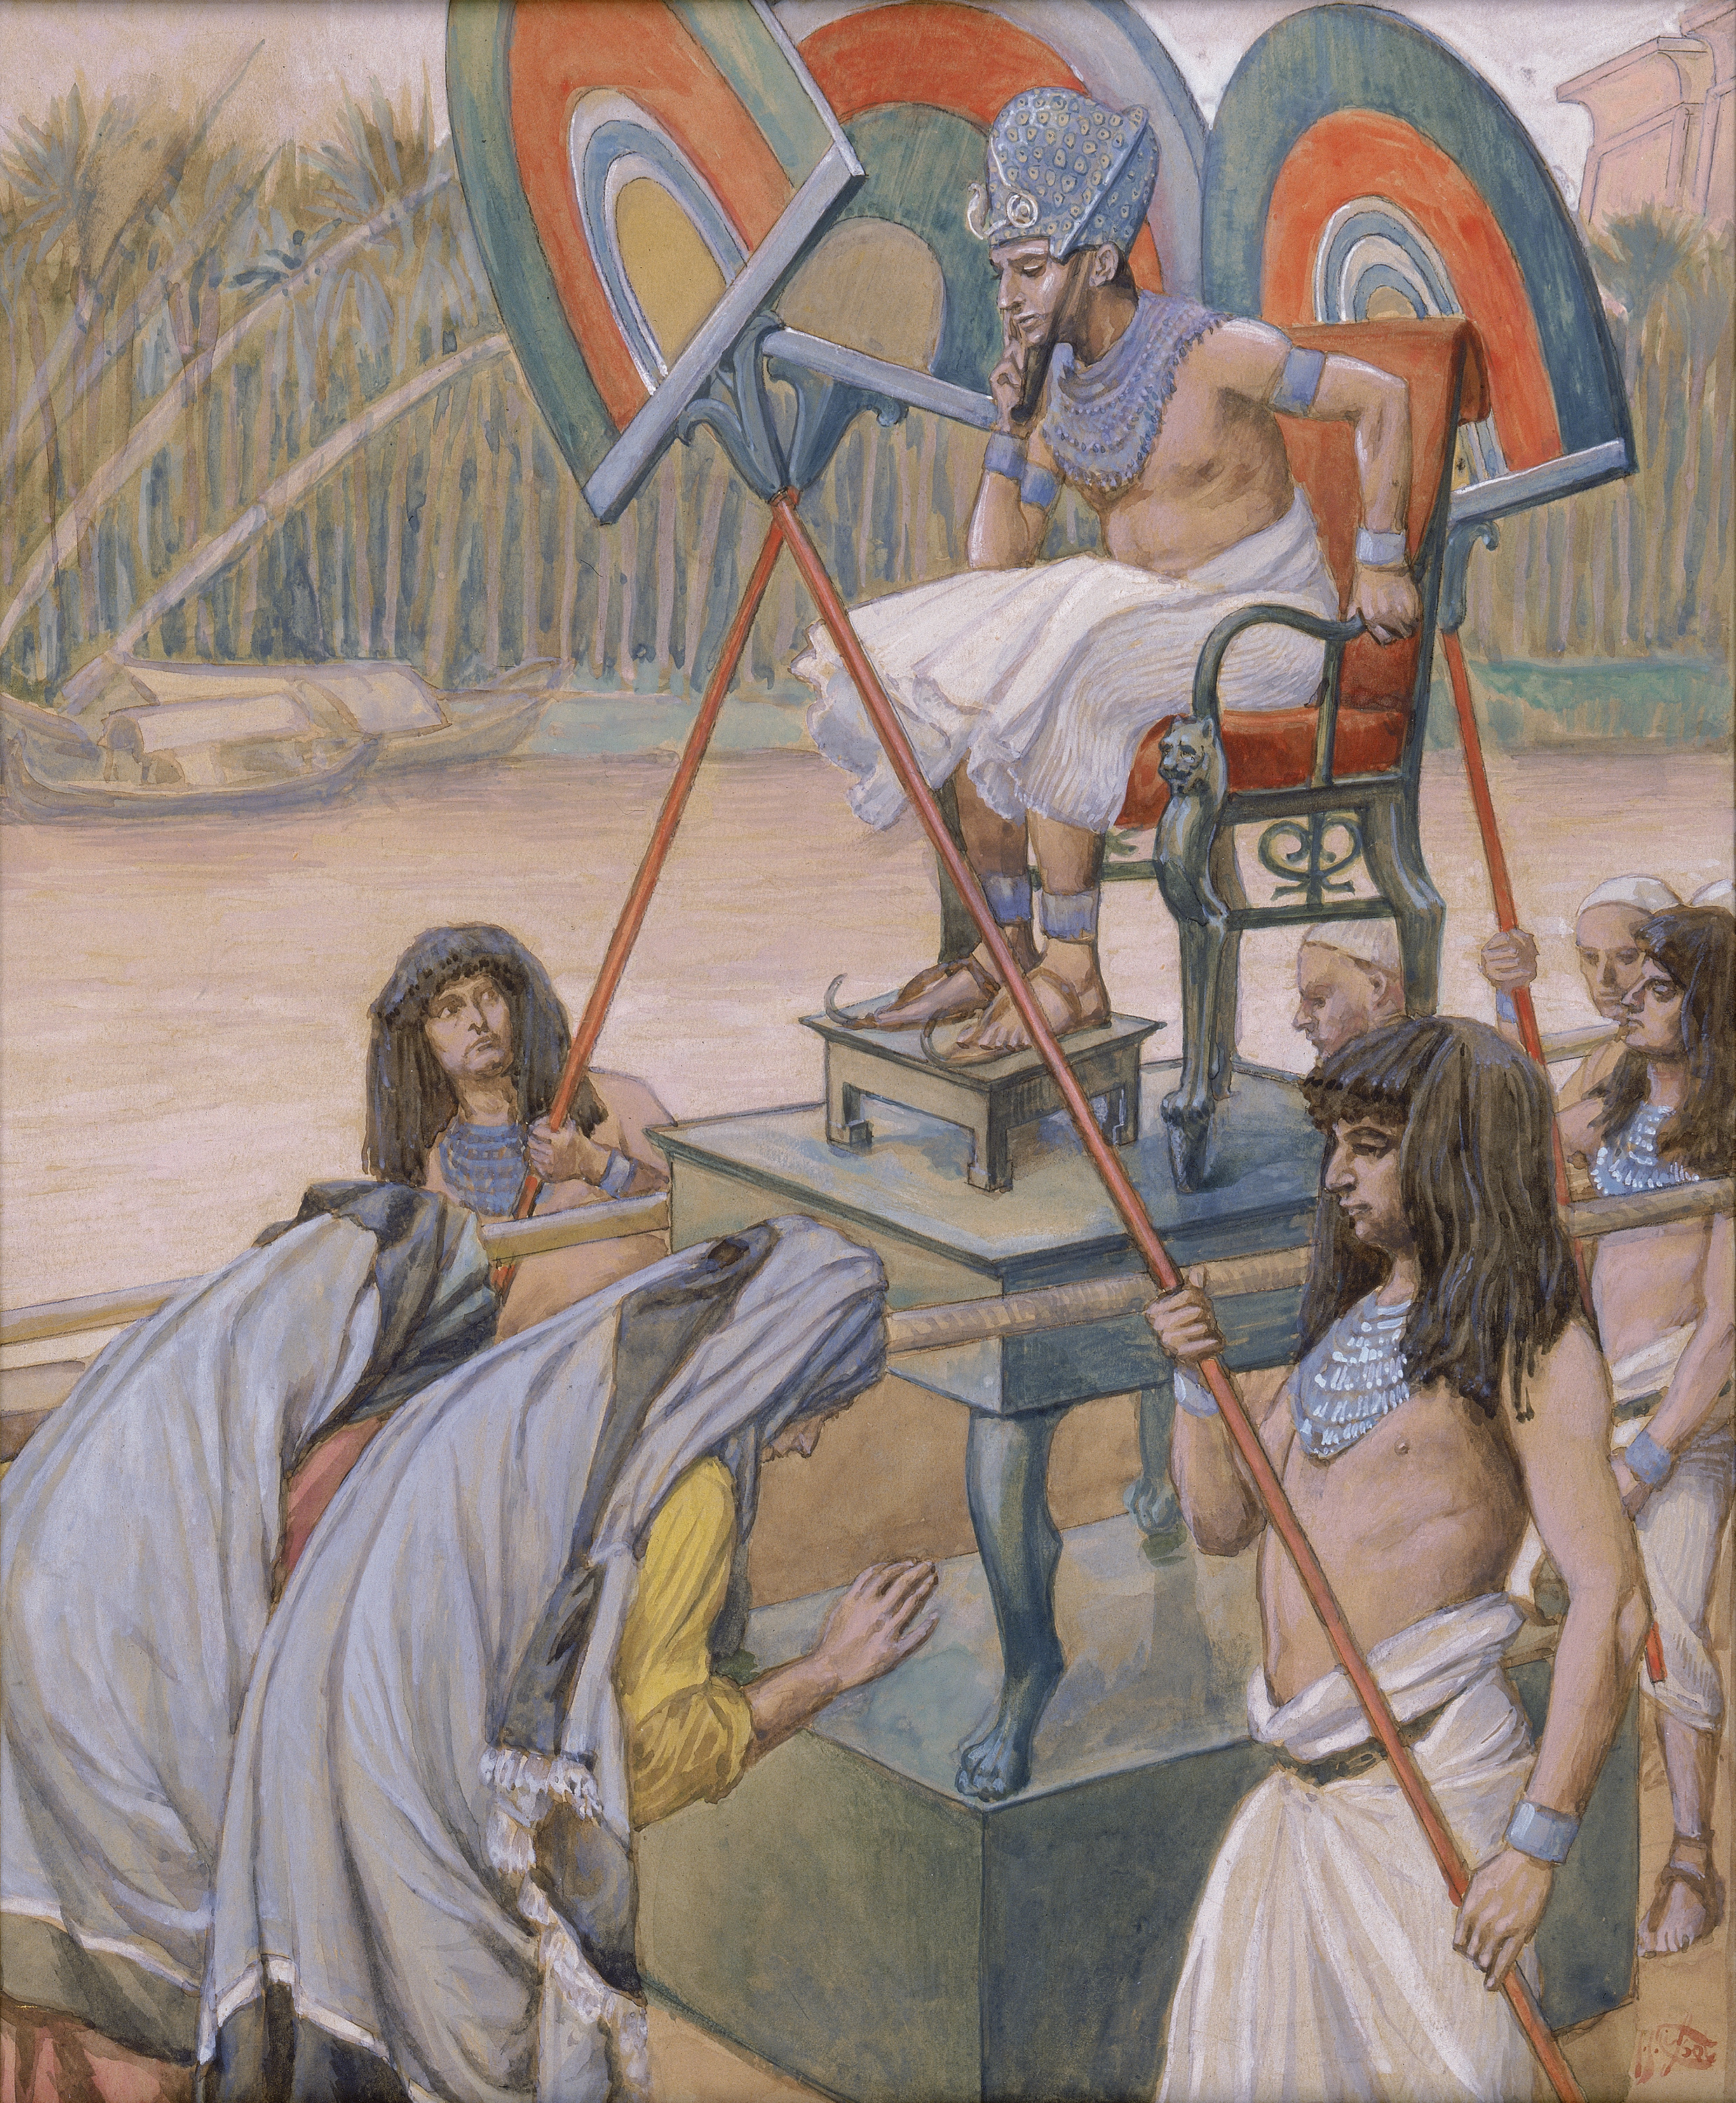
\includegraphics[width=1.3\linewidth]{midwives}}
%    }
%    \caption{\hspace*{-4.5cm}Obstetricēs et Rēx}
%\end{figure}

\titleimg{mw2.jpg}

{\begin{center}\large\bf\underline{Capitulum Primum}\end{center}%}

[In Aegyptō] fīliī Isrāēl crēvērunt, et \marginpar{quasi germinantēs: non vero germinantēs (quia hominēs non germinant) sed vidērī aliquō modō germināre}quasi\marginpar{germināre: emittere germina (ea quae ex plantīs veniunt: semen, fructus, cēt.)} germinantēs \marginpar{multiplicāre: multum facere; augēre}multiplicātī sunt:
ac rōborātī \marginpar{rōborāre: virēs dāre}nimis, implēvērunt terram.

Surrēxit intereā rēx novus super Ægyptum, quī ignōrābat Ioseph.
Et ait ad populum suum: ``Ecce, populus fīliōrum Isrāēl multus, et fortior nōbīs est.
Venīte, \marginpar{{\bf sapienter (adv) <} sapiēns}\marginpar{opprimere: efficere ut aliquis surgere nōn potest}\marginpar{ingruere: cum vi accedere}sapienter opprimāmus eum, nē forte multiplicētur: et sī ingruerit contrā nōs bellum, addātur inimīcīs nostrīs, expugnātisque nōbīs ēgrediātur dē terrā.''

\begin{figure}[h]
    \begin{minipage}[h]{0.5\linewidth}
        \centering
        
\includegraphics{tab}
        \caption{tabernaculum, -ī (n)}
    \end{minipage}%
    \begin{minipage}[h]{0.5\linewidth}
        \vspace*{-0.3cm}
        \centering
        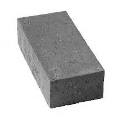
\includegraphics{later}
        \vspace*{-0.425cm}
        \caption{later, lateris (m)}
    \end{minipage}
\end{figure}

Præposuit \marginpar{praeposuit eīs magistrōs operum: dedit magistrīs potestatem super opera fīliōrum Isrāēl}itaque eīs magistrōs operum, ut afflīgerent eōs \marginpar{onus, oneris (n): res quam difficile est portare vel agere. e.g: saccus lapidibus plenus, labor difficilis} oneribus: 
ædificaveruntquē urbēs tabernāculōrum Pharaōnī, Phithom et Ramessēs.
Quantōque opprimēbant eōs, tantō magis multiplicābantur, et crēscēbant: 
ōderantque fīliōs Isrāēl Ægyptiī, et afflīgēbant \marginpar{illūdere: deridēre}illūdentēs eīs,
atque ad \marginpar{{\bf amāritūdo, -inis (f)}\\\hspace{0.5cm} < amārus/a/um $\leftrightarrow$ dulcis, -e}amāritūdinem \marginpar{per-dūcere: trahere}perdūcēbant vītam eōrum operibus dūrīs \marginpar{lutum, -ī(n): terra humida}lutī et lateris, omnīque \marginpar{famulātus, -ūs (m): servitus; conditiō servōrum}famulātū, quō in terræ operibus premēbantur. 
Dīxit autem rēx Ægyptī \marginpar{obstetrix, -īcis(f): femina quae iuvat feminam gravidam parere} obstetrīcibus Hebræōrum, quārum ūna vocābātur Sephora, altera Phua, 
\marginpar{praecipere: imperāre} præcipiēns eīs: ``Quandō obstetrīcābitis Hebræās, et \marginpar{partus, -ūs (m): actus pariendi} partus tempus advēnerit: sī masculus fuerit, interficite eum: sī fēmina, \marginpar{reservāre: servāre, conservāre}reservātē.''

Timuērunt autem obstetrīcēs Deum, \marginpar{praeceptum, -ī: quod praecipitur}\marginpar{nōn fēcērunt iuxtā praeceptum regis: non parent praeceptō rēgis}et nōn fēcērunt iuxtā præceptum rēgis Ægyptī, sed \marginpar{cōnservāre: servāre}cōnservābant \marginpar{mas, maris(m): homo (vel animal) masculinus}marēs. 
Quibus ad sē accersītis, rēx ait: ``Quidnam est hoc quod facere voluistis, ut puerōs servārētis?''

Quæ respondērunt: ``Nōn sunt Hebreæ sīcut Ægyptiæ mulierēs: ipsæ enim obstetrīcandī habent \marginpar{scientia, -ae (f) (< scīre): id quod scītur}scientiam, et priusquam veniāmus ad eās, pariunt.''

Bene ergō fēcit Deus obstetrīcibus: et crēvit populus, \marginpar{cōnfortāre: fortem facere, consolārī}cōnfortātusque est nimis.
Et quia timuērunt obstetrīcēs Deum, ædificāvit eīs domōs.
Præcēpit ergō Pharaō omnī populō suō, dīcēns: ``Quidquid masculīnī sexūs nātum fuerit, in flūmen prōiicite: quidquid fēminīnī, reservātē.''

%\section{Quaestiō Augustīnī}

{\it Dē obstetrīcum mendāciō, quō fefellērunt Pharaōnem, nē
occīderent masculōs Isrā-ēlītās quandō nāscēbantur, dīcentēs
nōn ita pārēre mulierēs Hebraēās sīcut pariēbant Aegyptiae:}

\mimg{aug.jpg}{Augustinus}Quaerī solet utrum tālia mendācia approbāta sint
auctōritāte dīvīnā, quandōquidem scrīptum est Deum
bene fēcisse obstetrīcibus: sed utrum prō misericordiā
ignōscēbat mendāciō; an et ipsum mendācium dignum
praemiō iūdicābat, incertum est.

\marginpar{vīvificāre: vivum facere, vitam dare}Aliud enim faciēbant obstetrīcēs vīvificandō
īnfantēs parvulōs, aliud Pharaōnī mentiendō: nam
in illīs vīvificandīs opus misericordiae fuit; mendāciō
vērō illō prō sē ūtēbantur, nē nocēret illīs
Pharaō, quod potuit nōn ad laudem, sed ad veniam pertinēre.

\marginpar{id est, ut ita dīcam, haec fābula nōn dat licentiam mentiendī}Neque hinc auctōritātem ad mentiendum esse prōpositam
\marginpar{eōrum: sanctōrum}mihi vidētur eīs dē quibus dictum est: ``Et nōn est
inventum in ōre eōrum mendācium.''

Quōrumdam enim vīta longē
īnferior ā professiōne sānctōrum, sī habeat ista
mendāciōrum peccāta, prōvectū ipsō et indole feruntur,
\marginpar{{\bf nōrunt} = nōvērunt}praesertim sī beneficia dīvīna nōndum nōrunt exspectāre
coelestia, sed circā terrēna occupantur.

\marginpar{conversātiō, -ōnis (f): modus vīvendī}Quī autem ita vīvunt, ut eōrum conversātiō,
sīcut dīcit Apostolus,
in coelīs sit, nōn eōs exīstimō linguae suae modum,
\marginpar{non exīstimō eōs debēre formāre modum linguae suae exemplō illō obstetrīcum}
quantum ad vēritātem prōmendam attinet falsitātemque vītandam,
exemplō illō obstetrīcum dēbēre fōrmāre.

\marginpar{disserere: sermōnem īnstituere dē rē aliquā, dīcere, disputāre, tractāre}Sed dīligentius dē hāc quaestiōne disserendum est,
propter alia exempla quae in Scrīptūrīs reperiuntur.


\chapter{}

\titleimg{baby2.jpg}

\mktitle{Capitulum Secundum}
\thispagestyle{empty}

\vnum{1}Ēgressus est post hæc vir dē domō Levī: et accēpit uxōrem \mpp{stirps, stirpis (m/f):}{e.g, frater matris est `stirpis meae', filia sororis patris quoque est `stirpis meae'. Quisquis ex familiā meā est, `stirpis meae' vocatur}stirpis suæ.
\vnum{2}Quæ \mpp{concipere:}{femina quae concipit efficit ut infans in eā incipit crescere}concēpit, et peperit fīlium: et vidēns eum \mpp{ēlegāns =}{pulcher}ēlegantem, abscondit tribus mēnsibus.
\mpp{scirpeus/a/um:}{ex scirpīs factus}
\mpp{līnere:}{ponere rem mollem premendō ac tergendō}
\mpp{bitūmen, -inis (n):}{māteria mollis atque ātra in terrā inventa quae pōnitur in rēbus nē aqua īnfluere possit}


\begin{figure}[hp]
    \begin{minipage}[hbp]{0.5\linewidth}
        \centering
        \includegraphics{basket}
        \caption{fiscella, -ae (f)}
    \end{minipage}%
    \begin{minipage}[hbp]{0.5\linewidth}
        \centering
        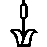
\includegraphics{brush}
        \caption{scirpus, -ī (m)}
    \end{minipage}
\end{figure}

\vnum{3}Cumque iam cēlāre nōn posset, sūmpsit fiscellam scirpeam,
et līnīvit eam bitūmine ac \mpp{pix, picis (f):}{māteria bitūminī similis mollis atque ātra ex parte arboris facta}pice:
posuitque intus īnfantulum, et exposuit eum in \mpp{cārex, cāricis (f):}{herba acuta et durissima}\mpp{cārectum, -ī (n):}{locus caricibus plenus}cārectō \mpp{rīpa, -ae (f):}{terra tangēns flumen}
rīpæ flūminis,
\vnum{4}stante procul sorōre eius, et \mpp{cōnsīderāns ēventum reī:}{exspectans ut videat quid futurum sit}
cōnsīderante ēventum reī.
\vnum{5}Ecce autem dēscendēbat fīlia Pharaōnis ut lavārētur in flūmine.\mpp{crepīdo, -inis (f):}{ripa fluminis lapidibus strata}\mpp{alveus, -ī (m):}{fossa per quam fluvius fluit} Et puellæ eius \mpp{gradī:}{gradum facere, ambulāre}gradiēbantur per crepīdinem alveī.
\mpp{papyrio, -ōnis (m):}{locus multīs cum papyrīs}Quæ cum vīdisset fiscellam in papȳriōne,
mīsit ūnam ē \mpp{famula, -ae (f):}{ancilla}famulābus suīs: et allātam \vnum{6}aperiēns,
cernēnsque in eā parvulum vāgientem,
\mpp{miserta (+ gen.):}{tristis propter aliquem miserum}miserta eius, ait: ``Dē īnfantibus Hebræōrum est hic.''

\vnum{7}Cui soror puerī: ``Vīs,'' inquit, ``ut vādam, et vōcem tibi mulierem Hebræam,
quæ \mpp{nūtrīre:}{dāre lac}nūtrīre possit \mpp{īnfantulus/a/um:}{parvus īnfans}īnfantulum?''\mimg{papyrus}{papyrus, -ī (m/f)}

\vnum{8}Respondit: ``Vāde.''

Perrēxit puella et vocāvit mātrem suam.
\vnum{9}Ad quam locūta fīlia Pharaōnis: ``Accipe,'' ait, ``puerum istum, et nūtrī mihi: ego dabō tibi mercēdem tuam.''

\mpp{suscipere:}{sumere, capere}Suscēpit mulier, et nūtrīvit puerum: \mpp{adultus/a/um:}{iam vir/femina, non puer/puella}adultumque trādidit fīliæ Pharaōnis. 
\mpp{adoptāre:}{qui adoptat aliquem facit eum filium vel filiam suam}\vnum{10}Quem illa adoptāvit in locum fīliī,
vocāvitque nōmen eius Moysēs, dīcēns: ``Quia dē aquā tulī eum.''

\vnum{11}In diēbus illīs postquam crēverat Moysēs, ēgressus est ad frātrēs suōs:
\mpp{percutere:}{pulsare, afficere, et quasi vulnerare dolore}vīditque afflīctiōnem eōrum et virum Ægyptium percutientem quemdam dē Hebræīs frātribus suīs.
\vnum{12}Cumque circumspexisset hūc atque illūc,
et nūllum adesse vīdisset,
\mimg{sabulum}{sabulum, -ī (n)}\mpp{abscondere:}{rem in aliquo loco ponere ut celetur}
percussum Ægyptium abscondit sabulō.
\mpp{rixāre:}{certāre}

\vnum{13}Et ēgressus diē alterō cōnspexit duōs Hebræōs rixantēs:
dīxitque eī quī faciēbat iniūriam: ``Quārē percutis proximum tuum?''

\mpp{prīnceps, prīncipis (m):}{rex; dux}\vnum{14}Quī respondit: ``Quis tē cōnstituit prīncipem et \mimg{judge_small}{\hspace*{0.75cm}iūdex, iūdicis (m/f)}iūdicem super nōs?
Num occīdere mē tū vīs, sīcut heri occīdistī Ægyptium?''

\mpp{palam}{$\leftrightarrow$ occulte}Timuit Moysēs, et ait: ``Quōmodo palam factum est verbum istud?''

\vnum{15}Audīvitque Pharaō sermōnem hunc, et quærēbat occīdere Moysēn:
quī fugiēns dē cōnspectū eius, morātus est in terrā Madiān,
\mimg{puteus.png}{puteus, -ī (m)}et sēdit iuxtā puteum.
\vnum{16}Erant autem sacerdōtī Madian septem fīliæ,
quæ vēnērunt ad \mpp{haurīre:}{sumere ex loco ubi aqua est}hauriendam aquam:
\mpp{adaquāre:}{aquam dāre}et implētīs \mpp{canālis, -is (m/f):}{rēs in quam aqua funditur ut animal bibat}canālibus adaquāre cupiēbant gregēs patris suī.
\mpp{supervēnīre:}{subitō adesse nocendī causā}\mpp{supervēnēre =}{supervēnērunt}\vnum{17}Supervēnēre pāstōrēs, et ēiēcērunt eās:
surrēxitque Moysēs, et dēfēnsīs puellīs, adaquāvit ovēs eārum. 
\vnum{18}Quæ cum revertissent ad Raguel patrem suum, dīxit ad eās:
\mpp{vēlox, -ōcis:}{celer}``Cūr vēlōcius vēnistis solitō?''

\vnum{19}Respondērunt: ``Vir Ægyptius līberāvit nōs dē manū pāstōrum:
\mpp{īnsuper:}{praeterea}īnsuper et hausit aquam nōbīscum, \mpp{pōtus, -ūs (m):}{pōtiō}pōtumque dedit ovibus.''

\vnum{20}At ille: ``Ubi est?'' inquit: ``Quārē dīmīsistis hominem? Vocātē eum ut \mpp{comedere:}{totum ēsse; ēsse}comedat pānem.''

\vnum{21}Iūrāvit ergō Moysēs quod habitāret cum eō.
Accēpitque Sephoram fīliam eius uxōrem:
\vnum{22}Quæ peperit eī fīlium, quem vocāvit Gersam, dīcēns:
\mpp{advena, -ae (m)}{quī nōn est cīvis, qui ab aliō locō venit}``Advena fuī in \mpp{terra aliēna:}{terra ubi is nōn natus est}terrā aliēnā.''

Alterum vērō peperit, quem vocāvit Eliezer, dīcēns:
\mpp{adiūtor, -ōris (m):}{qui adiuvat}``Deus enim patris meī adiūtor meus ēripuit mē dē manū Pharaōnis.''

\vnum{23}Post multum vērō tempore mortuus est rēx Ægyptī:
\mpp{ingemīscere:}{dolēre}et ingemīscentēs fīliī Isrāēl
propter opera vōciferātī sunt:
\mpp{vōciferātus/a/um $<$ vōciferārī:}{valde exclamāre}
ascenditque clāmor eōrum ad Deum ab operibus.
\mpp{gemitus, -ūs (m):}{sonus atque actus dolendī}\vnum{24}Et audīvit gemitum eōrum,
\mpp{pangō, pangere, pepigisse, pactum:}{constituere, statuere}ac \mpp{recordor, -ārī, -ātus sum:}{meminisse}recordātus est fœderis quod pepigit cum Abraham, Isaac et Iācōb.
\mpp{respicere:}{aspicere iuvandī causā}\vnum{25}Et respexit Dominus fīliōs Isrāēl et cognōvit eōs.

%\section{Quaestiō Augustīnī}

\mimg{aug.jpg}{Augustinus}{\it Dē factō Moȳsī, cum occīdit Aegyptium ad dēfendendōs
frātrēs suōs: utrum indolēs in eō laudābilis fuerit,
\marginpar{admittere: permittere}\marginpar{ūber, ūberis (n): fertilitas, fecunditas}
\marginpar{ferācitas, -ātis (f): fertilitas, fecunditas}quā hoc peccātum admīserit, sīcut solet ūber terrae,
\marginpar{id est, vidimus terram herbārum inūtilium plēnam et dicimus, ``Ecce! Tam fertilis terra!'' -- res mala (herbae inūtiles) est signum reī bonae (fertilitatis)}etiam ante ūtilia sēmina, quādam herbārum quamvīs
inūtilium ferācitāte laudārī;
an omnīnō ipsum factum iustificandum sit.}

\marginpar{lēgitimus/a/um: qui secundum leges est}Quod ideō nōn vidētur, quia nūllam adhūc lēgitimam
\marginpar{dīvīnitus (adv): ā Deō}potestātem gerēbat, nec acceptam dīvīnitus, nec
hūmānā societāte ōrdinātam.

Tamen, sīcut Stephanus
dīcit in Āctibus Apostolōrum, putābat intellegere
frātrēs suōs, quod per eum Deus daret illīs
salūtem: ut per hoc testimōnium videātur
Moysēs iam dīvīnitus admonitus (quod
Scrīptūra eō locō tacet) hoc audēre potuisse.


\chapter{}

\titleimg{bush2.jpg}
\thispagestyle{empty}

\mktitle{Capitulum Tertium}
\vspace*{-0.75cm}
Moysēs autem pāscēbat ovēs Iethrō \mpp{socer, socerī:}{pater uxōris vel pater marītī}suī sacerdōtis Madian:
\mpp{mināre:}{cōgere animālia}cumque mināsset gregem ad \mpp{interiōr, -ōris (adj.):}{magis intus}interiōra \mpp{dēserta, -ōrum (n):}{locus ubi paene nihil est; locus sine imbre et aquā}dēsertī,
venit ad montem Deī Horeb.
\mpp{rubus, -ī (m):}{quaedam herba}
Appāruitque eī Dominus in flammā ignis dē mediō rubī:
et vidēbat quod rubus \mpp{ārdēre:}{habēre ignem in sē}ārdēret, et nōn \mpp{combūrere:}{igne perdere}combūrerētur.
Dīxit ergō Moysēs: \mpp{vādere:}{īre, ambulāre}``Vādam, et vidēbō \mpp{vīsiō, -ōnis (f):}{quod vīsum est; āctus videndī}vīsiōnem hanc magnam, quārē nōn combūrātur rubus.''

Cernēns autem Dominus quod pergeret ad videndum,
vocāvit eum dē mediō rubī, et ait: ``Moysēs, Moysēs.''

Quī respondit: ``Adsum.''

At ille: ``Nē \mpp{appropiāre =}{adīre}appropiēs,'' inquit, ``hūc: solve \mpp{calceāmentum:}{quod pedī induitur}calceāmentum dē pedibus tuīs: locus enim
in quō stās \mpp{terra sāncta:}{terra deō cōnstitūta}terra sāncta est.'' 

Et ait: ``Ego sum Deus patris tuī, Deus Abraham, Deus Isaac et Deus Iācōb.''

Abscondit Moysēs faciem suam: nōn enim audēbat aspicere contrā Deum.

Cui ait Dominus: ``Vīdī \mpp{afflīctiō, -ōnis (f):}{rēs quae nocet vel valde non placet}afflīctiōnem populī meī in Ægyptō,
et clāmōrem eius audīvī propter \mpp{duritia, -ae (f) $<$}{durus/a/um}dūritiam eōrum quī \mpp{prae-esse:}{esse prae alios; dux esse}præsunt operibus:
et sciēns dolōrem eius, dēscendī ut libērem eum dē manibus Ægyptiōrum,
et ēdūcam dē terrā illā in terram bonam, et \mpp{spatiōsus/a/um:}{magnus}spatiōsam,
in terram quæ fluit lacte et melle,
\mpp{loca =}{locī (nom. pl.)} ad loca Chananæī et Hethæī, et Amorrhæī, et Pherezæī, et Hevæī, et Iebusæī.
Clāmor ergō fīliōrum Isrāēl venit ad mē: vīdīque afflīctiōnem eōrum,
qua ab Ægyptiīs \mpp{opprimere:}{efficere ut aliquis surgere nōn possit}opprimuntur.
Sed vēnī, et mittam tē ad Pharaōnem,
ut ēducās populum meum, fīliōs Isrāēl, dē Ægyptō.''

Dīxitque Moysēs ad Deum: ``Quis sum ego ut vādam ad Pharaōnem,
et ēdūcam fīliōs Isrāēl dē Ægyptō?''

Quī dīxit eī: ``Ego erō tēcum: et hoc habēbis signum,
quod mīserim tē: cum ēdūxerīs populum meum dē Ægyptō,
immolābis Deō super montem istum.''

Ait Moysēs ad Deum: ``Ecce ego vādam ad fīliōs Isrāēl,
et dīcam eīs: Deus patrum vestrōrum mīsit mē ad vōs.
Sī dīxerint mihi: `Quod est nōmen eius?' quid dīcam eīs?''

Dīxit Deus ad Moysēn: ``EGO SUM QUĪ SUM.'' Ait: ``Sīc dīcēs fīliīs Isrāēl: `QUĪ EST mīsit mē ad vōs.' ''

Dīxitque iterum Deus ad Moysēn: ``Hæc dīcēs fīliīs Isrāēl:
Dominus Deus patrum vestrōrum, Deus Abraham, Deus Isaac et Deus Iācōb,
\mpp{in æternum:}{semper} mīsit mē ad vōs: hoc nōmen mihi est in æternum,
\mpp{memoriāle, -is (n):}{id quod memorandum est}et hoc memoriāle meum in generātiōnem et generātiōnem.''

``Vāde, et \mpp{congregāre:}{in unum locum cōgere vel ferre vel ducere}, congregā \mpp{seniōr, -ōris (adj):}{magis senex; hīc seniōrēs virī, id est, principēs}seniōrēs Isrāēl,
et dīcēs ad eōs: Dominus Deus patrum vestrōrum appāruit mihi,
Deus Abraham, Deus Isaac et Deus Iācōb,
\mpp{vīsitāre:}{vīsum īre}dīcēns: Vīsitāns vīsitāvī vōs: et vīdī omnia quæ accidērunt vōbīs in Ægyptō.
Et dīxī ut ēdūcam vōs dē \mpp{afflīctiō, -ōnis (f):}{rēs quae nocet vel valde non placet}afflīctiōne Ægyptī in terram Chananæī,
et Hethæī, et Amorrhæī, et Pherezæī, et Hevæī, et Iebusæī,
ad terram fluentem lacte et melle.''

``Et audient vōcem tuam: ingrediērisque tū,
et seniōrēs Isrāēl, ad rēgem Ægyptī, et dīcēs ad eum:
Dominus Deus Hebræōrum vocāvit nōs:
ībimus viam trium diērum in \mpp{sōlitūdo, -inis ($<$ solus/a/um):}{deserta; locus ubi nemo vel unus habitat}sōlitūdinem,
\mpp{immolāre:}{sacrificium facere}ut immolēmus Dominō Deō nostrō.''

``Sed ego sciō quod nōn dīmittet vōs rēx Ægyptī
ut eātis nisi per manum validam.
Extendam enim manum meam, et percutiam Ægyptum
in cūnctīs mīrābilibus meīs, 
quæ factūrus sum in mediō eōrum:
post hæc dīmittet vōs.
Dabōque grātiam populō huic cōram Ægyptiīs:
\mpp{vacuuus/a/um:}{sine rēbus (cibō, vestimentīs, pecuniā)}et cum ēgrediēminī, nōn exībitis vacuī:
\mpp{vīcīnus/a:}{qui prope habitat}sed postulābit mulier ā vīcīnā suā
et ab hospitā suā, vāsa argentea et aurea, ac vestēs:
\mpp{spoliāre:}{capere rēs aliōrum hominum}pōnētisque eās super fīliōs et fīliās vestrās, et spoliābitis Ægyptum.''

%\section{Quaestiō Augustīnī}

\mimg{aug.jpg}{Augustinus}``Clāmāvit illum Dominus dē rubō.''

\marginpar{in angelō: in formā angelī (?)}Dominus in angelō an Dominus, angelus ille quī dictus est: 
``Magnī cōnsiliī angelus,'' (Isa 9:6) et intellegitur Chrīstus? 
Suprā enim dīxit: ``Appāruit illī angelus Dominī in flammā ignis dē rubō.''

\section{Quaestiō Augustinī Altera}

``Ēdūcere illōs dē terrā illa in terram bonam et
multam, in terram fluentem lac et mel.'' 

\marginpar{spīritāliter (adv.): secundum spiritum}Utrum terram fluentem lac et mel spīritāliter accipere
\marginpar{proprietas (verborum): conjunctio illorum arta et apta cum rebus ipsis, quas significant}dēbēmus? quia secundum proprietātem nōn hoc erat
illa quae data est populō Isrāēl? 
an locūtiōnis est, quā id ad laudem ūbertātis et suāvitātis referātur?


\chapter{}

\titleimg{inn.png}

{\begin{center}\large\bf\underline{Capitulum Quartum}\end{center}}
\vspace*{-1.0cm}

Respondēns Moysēs ait: ``Nōn crēdent mihi, neque audient vōcem meam, sed dīcent:
Nōn appāruit tibi Dominus.''

Dīxit ergō ad eum: ``Quid est quod tenēs in manū tuā?''

Respondit: ``Virga.''

\marginpar{prōiicere: procul iacere; abiicere} Dīxitque Dominus: ``Prōiice eam in terram.''

Prōiēcit, et versa est in colubrum, ita ut fugeret \marginpar{coluber, -brī (m): serpens}Moysēs. 

Dīxitque Dominus: ``Extende manum tuam, et apprehende caudam eius.''

Extendit, et tenuit, versaque est in virgam.
``Ut crēdant,'' inquit, ``quod appāruerit tibi Dominus Deus patrum suōrum,
Deus Abraham, Deus Isaac et Deus Iācōb.''

Dīxitque Dominus rūrsum: ``Mitte manum tuam in sinum tuum.''

\marginpar{{\bf leprōsus/a/um $<$ leprae, -ārum (f)}: morbus qui cutem (exterior pars hominis) deformat}
\marginpar{īnstar + gen: sicut}Quam cum mīsisset in sinum, prōtulit leprōsam īnstar nivis.
``Retrahe,'' ait, ``manum tuam in sinum tuum.''

Retrāxit, et prōtulit iterum,
et erat similis carnī reliquæ.
``Sī nōn crēdiderint,'' inquit, ``tibi, neque audierint
sermōnem signī priōris, crēdent verbō signī sequentis. 
Quod sī nec duōbus quidem hīs signīs crēdiderint,
neque audierint vōcem tuam: sūme aquam flūminis,
\marginpar{āridus/a/um: sine aquā}et effunde eam super āridam, et quidquid hauserīs dē fluviō,
vertētur in sanguinem.''

\marginpar{nūdiustertius: ante duōs diēs}
Ait Moysēs: ``Obsecrō, Domine, nōn sum ēloquēns ab heri et
\marginpar{{\bf ex quō} (tempore)}nūdiustertius: et ex quō locūtus es ad servum tuum,
impedītiōris et tardiōris linguæ sum.''

Dīxit Dominus ad eum: ``Quis fēcit os hominis?
\marginpar{fabricatus/a/um: confectus}
\marginpar{mūtus/a/um: loquī non potest}
\marginpar{surdus/a/um: audīre non potest}
aut quis fabricātus est mūtum et surdum,
\marginpar{caecus/a/um: vidēre non potest}videntem et cæcum? nōnne ego?
Perge, igitur, et ego erō in ōre tuō:
docēbōque tē quid loquāris.''

\marginpar{obsecrāre: orāre, precārī}At ille: ``Obsecrō, inquit, Domine,
mitte quem missūrus es.''

Īrātus Dominus in Moysēn, ait: ``Aarōn frāter tuus Lēvītēs,
sciō quod ēloquēns sit: ecce ipse ēgreditur in occursum tuum,
vidēnsque tē lætābitur corde.
Loquere ad eum, et pōne verba mea in ōre eius:
et ego erō in ōre tuō, et in ōre illīus,
et ostendam vōbīs quid agere dēbeātis.
Ipse loquētur prō tē ad populum,
et erit os tuum:
tū autem eris eī in hīs quæ ad Deum pertinent.
Virgam quoque hanc sūme in manū tuā,
in quā factūrus es signa.

\marginpar{socer, socerī (m): pater uxōris}Abiit Moysēs, et reversus est ad Iethrō socerum suum,
dīxitque eī: ``Vādam et revertar ad frātrēs meōs in Ægyptum,
ut videam sī adhūc vīvant.''

Cui ait Iethrō: ``Vāde in pāce.''

Dīxit ergō Dominus ad Moysēn in Madiān: ``Vāde, et revertere in Ægyptum,
mortuī sunt enim omnēs quī quærēbant animam tuam.''

\begin{figure}[hbp]
        \centering
        \setlength{\fboxsep}{0pt}
        \fbox{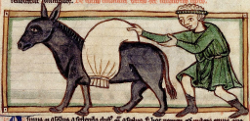
\includegraphics{asinus}}
        \caption{asinus, -ī (m)}
\end{figure}
Tulit ergō Moysēs uxōrem suam, et fīliōs suōs,
et imposuit eōs super asinum: reversusque est in Ægyptum,
portāns virgam Deī in manū suā. Dīxitque eī Dominus revertentī
in Ægyptum: ``Vidē ut omnia ostenta quæ posuī in manū tuā
\marginpar{indūrāre: durum facere}faciās cōram Pharaōne: ego indūrābō cor eius,
et nōn dīmittet populum. Dīcēsque ad eum: Hæc
\marginpar{prīmōgenitus: natū maior}dīcit Dominus: Fīlius meus prīmōgenitus Isrāēl.
Dīxī tibi: Dīmitte fīlium meum ut serviat mihi;
et nōluistī dīmittere eum:
ecce ego interficiam fīlium tuum prīmōgenitum.''

\marginpar{dīversōrium, -ī (n): aedificium in quō hominēs in itinere possunt dormīre}\marginpar{petra, -ae (f): lapis}Cumque esset in itinere, in dīversōriō
occurrit eī Dominus, et volēbat occīdere eum. 
\marginpar{idcircō: proptereā, ideō}Tulit idcircō Sephora acūtissimam petram,
\marginpar{praepūtium, -ī (n): illa pars puerī quae circumcīditur}et circumcīdit præpūtium fīliī suī, tetigitque pedēs ejus,
\marginpar{spōnsus/a: quī mox alicui maritus vel uxor erit}et ait: ``Spōnsus sanguinum tū mihi es.''
Et dīmīsit eum postquam dīxerat: ``Spōnsus sanguinum ob circumcīsiōnem.''

Dīxit autem Dominus ad Aarōn: ``Vāde in occursum Moȳsī
in dēsertum.'' 

Quī perrēxit obviam eī in montem Deī, et ōsculātus est eum.
Nārrāvitque Moysēs Aarōn omnia verba Dominī quibus miserat eum,
et signa quæ mandāverat. Vēnēruntque simul, et congregāvērunt
cūnctōs seniōrēs fīliōrum Isrāēl.
Locūtusque est Aarōn omnia verba quæ dīxerat Dominus ad Moysēn: et
fēcit signa cōram populō, et crēdidit populus.
Audiēruntque quod vīsitāsset Dominus fīliōs Isrāēl,
\marginpar{prōnus/a/um: iacēns in pectore}et respexisset afflīctiōnem illōrum: et prōnī adōrāvērunt.

%\section{Quaestiō Augustīnī}

Quemadmodum possit intellegī īrāscēns\linebreak
Deus, quia nōn sīcut homō per irratiōnābilem perturbātiōnem, per omnia
tenendum est, ubi tāle aliquid Scrīptūra dīcit, nē dē hōc eadem saepe
\mimg{aug.jpg}{Augustinus}
dīcenda sint. Sed meritō quaeritur cūr hīc īrātus dē frātre Moyse
dīxerit, quod ipse illī loquerētur ad populum: vidētur enim tamquam
\marginpar{diffīdere: nōn fīdere}diffīdentī nōn dedisse plēnissimam facultātem, quam datūrus erat; et per 
duōs agī voluisse, quod et per ūnum posset, sī crēdidisset.

Vērumtamen
eadem verba omnia dīligentius cōnsīderāta, nōn significant īrātum
\marginpar{vindicta, -ae (f): ultio vel animadversio pro delicto;
vindicatio}Dominum prō vindictā dedisse Aarōn. Sīc enim dīcit: ``Nōnne ecce Aarōn
frāter tuus Lēvītēs? sciō quia loquēns loquētur ipse.''

Quibus verbīs
ostenditur Deus increpāsse potius eum, quī timēret īre quod ipse esset
minus idōneus, cum habēret frātrem per quem posset ad populum loquī quod
\marginpar{gracilis, -is (adj): tenuis, exilis}vellet; quoniam erat ipse gracilis vōcis, et linguae tardiōris: quamquam
dē Deō tōtum spērāre dēbēret. Deinde eadem ipsa quae paulō ante
prōmīserat, et posteāquam īrātus est, dīcit. Dīxerat enim: ``Aperiam os
tuum, et īnstruam tē''; nunc autem dīcit: ``Aperiam os tuum et os eius, et
īnstruam vōs quae faciātis''; sed quoniam addidit: ``Et loquētur ipse tibi
ad populum,'' vidētur ōris apertiō praestita, propter quod dīcit Moysēs
linguae sē esse tardiōris. 

Dē vōcis autem gracilitāte nihil eī praestāre
\marginpar{adiūtōrium, -ī (n): auxilium, quodqumque adiuvat}Dominus voluit, sed propter hoc adiūtōrium frātris adiūnxit, quī posset
eā utī vōce, quae pōpulō docendō sufficeret. Quod ergō ait: ``Et dabis
verba mea in os eius,'' ostendit quod ea loquenda esset datūrus: nam sī
\marginpar{tantummodo: solum, solummodo}tantummodo audienda, sīcut populō, in aurēs dīceret. Deinde quod paulō
post ait: ``Et loquētur ipse tibi ad populum, et ipse erit tuum os, et hic
subaudītur, ad populum.'' Et cum dīcit: ``Tibi loquētur ad populum''; satis
indicat in Moysēn prīncipātum, in Aarōn ministerium. Deinde quod ait: ``Tū
\marginpar{fortassis = fortasse}autem illī eris quae ad Deum,'' magnum
hīc fortassis perscrūtandum 
\marginpar{sacrāmentum, -ī: mysterium, signum sensibile rei sacrae
latentis}est sacrāmentum, cuius figūram gerat, velutī medius Moysēs inter Deum et
Aarōn, et medius Aarōn inter Moysēn et populum. 

\section{Quaestiō Augustīnī Altera}

\marginpar{obviāre: obviam īre}In eō quod scrīptum est: Et factum est, in viā ad refectiōnem obviāvit
\marginpar{calculus: parvus lapis}eī angelus, et quaerēbat eum occīdere: et assūmptō Sepphora calculō,
\marginpar{praepūtium, -ī (n): illa pars puerī quae circumcīditur}circumcīdit praepūtium fīliī suī; et prōcidit ad pedēs eius, et dīxit:
``Stetit sanguis circumcīsiōnis īnfantis meī. Et recessit ab eō;'' propter
quod dīxit: ``Dēsiit sanguis circumcīsiōnis;'' 

Prīmum quaeritur, quem
volēbat angelus occīdere, utrum Moysen, quia dictum est, ``occurrit eī
angelus, et quaerēbat eum occīdere.'' Nam cui putābitur occurrisse, nisi
\marginpar{comitātus, -ūs (m): comitum multitudo}illī quī ūniversō suōrum comitātuī praefuit, et ā quō caeterī
dūcēbantur? An puerum quaerēbat occīdere, cui māter circumcīdendō
\marginpar{subvenīre: opem ferre, auxiliari, succurrere}subvenit; ut ob hoc intellegātur occīdere voluisse īnfantem, quia nōn
\marginpar{sancīre: aliquid ritu sacro, seu religioso decernere,
constituere}erat circumcīsus, atque ita sancīre praeceptum circumcīsiōnis,
sevēritāte vindictae?

Quod sī ita est, incertum est prius dē quō
\marginpar{id est, ut ita dicam, quis est ``eum''? Quis est ``eī''?}dīxerit, ``quaerēbat eum occīdere;'' quia ignōrātur quem, nisi ex
cōnsequentibus reperiātur: mīrā sānē locūtiōne et inūsitātā, ut prius
dīceret, ``occurrit eī,'' et quaerēbat eum occīdere, dē quō nihil anteā
dīxerat.

Sed tālis est in Psalmō: ``Fundāmenta eius in montibus sānctīs;
dīligit Dominus portās Sīōn.'' Inde enim Psalmus incipit, nec aliquid
dē illō vel dē illā dīxerat, cuius fundāmenta intellegī voluit, dīcēns:
Fundāmenta eius in montibus sānctīs. Sed quia sequitur, ``dīligit Dominus
portās Sīōn,'' ergō fundāmenta vel Dominī vel Sīōn, et ad faciliōrem
sēnsum magis Sīōn, ut fundāmenta cīvitātis accipiantur. Sed quia in hōc
prōnōmine, quod est, ``eius,'' genus ambiguum est (omnis enim generis est
hoc prōnōmen, id est et masculīnī, et fēminīnī, et neutrī), in graecō
autem in fēminīnō genere ``autes'' dīcātur, masculīnō et neutrō
``autou'', et habet cōdex
graecus ``autou'', cōgit intellegere nōn fundāmenta Sīōn, sed fundāmenta Dominī,
id est, quae cōnstituit Dominus, dē quō dictum est: ``Aedificāns Ierusālem
Dominus.'' Nec Sīōn tamen, nec Dominum anteā nōmināverat, cum dīceret:
``Fundāmenta eius in montibus sānctīs.'' 

Sīc et hīc nōndum nōminātō īnfante
dictum est, ``occurrit eī, et quaerēbat eum occīdere;'' ut dē quō dīxerit,
in cōnsequentibus agnōscāmus.  Quamquam etsī dē Moyse accipere quisquam
\marginpar{magnopere: valde, vehementer}voluerit, nōn est magnopere resistendum.

Illud potius quod sequitur, sī
fierī potest, intellegātur, quid sibi velit ideō recessisse angelum ab
interfectiōne cuiuslibet eōrum, quia dīxit mulier: ``Stetit sanguis
circumcīsiōnis īnfantis.'' Nōn enim ait: Recessit ab eō, propter quod
circumcīdit īnfantem: sed quia stetit sanguis circumcīsiōnis; nōn quia
cucurrit, sed quia stetit: magnō, nisi fallor, sacrāmentō. 


\chapter{}
\titleimg{bricks.jpg}
\mktitle{Capitulum Quintum}
\thispagestyle{empty}

Post hæc \mpp{ingredī:}{intus īre}ingressī sunt Moysēs
et Aarōn, et dīxērunt Pharaōnī: ``Hæc dīcit Dominus Deus
Isrāēl: Dīmitte populum meum ut
\mpp{sacrificāre}{animal interficere vel rem offerre ut placeat deō}sacrificet mihi in dēsertō.''

At ille respondit: ``Quis est
Dominus, ut audiam vōcem eius, et dīmittam Isrāēl? Nesciō
Dominum, et Isrāēl nōn dīmittam.''

Dīxēruntque: ``Deus
Hebræōrum vocāvit nōs, ut eāmus viam trium diērum in
\mpp{sōlitūdō:}{deserta; locus ubi nemo vel unus habitat}sōlitūdinem, et
sacrificēmus Dominō Deō nostrō: nē forte accidat nōbīs
\mpp{pestis, -is (f):}{aliquid corporī malum: e.g, aeger fiērī}pestis aut
gladius.''

Ait ad eōs rēx Ægyptī: ``Quārē
Moysēs et Aarōn \mpp{sollicitāre:}{allicere}sollicitātis populum ab
operibus suīs? Īte ad \mpp{onus, oneris (n):}{res quae difficile est portare vel agere. e.g: saccus lapidibus plenus, labor difficilis}onera vestra.''

Dīxitque
Pharaō: ``Multus est populus terræ: vidētis quod turba
\mpp{succrēscere (sub + crēscere):}{ab īmō crēscere}succrēverit: quantō magis sī dederītis eīs
\mpp{requiēs, requieī (f):}{tempus quō homō non laborāt}requiem ab operibus?'' 

\kimg{palea}{paleam colligentes}

Præcēpit \mpp{praecipere:}{imperāre}ergō in diē illō
\mpp{praefectus, -ī (m):}{homo qui alicuī reī vel negotiō praepositus est}præfectīs operum et \mpp{exāctōr, -ī:}{quī facit ut opera perficiantur}exāctōribus populī,
dīcēns:  ``\mpp{nēquāquam:}{minimē, nullō modō}Nēquā\-quam ultrā dabitis paleās
populō ad cōnficiendōs laterēs, sīcut prius: sed ipsī \mpp{vadere:}{īre, ambulāre}vadant, et colligant \mpp{stipula, ae}{media ac longa pars herbae
ex quā aliae partēs extendunt}stipulās. 
Et \mpp{mēnsūra:}{e.g, si praefectus dicit ``pone centum laterēs in hōc
vase,'' centum laterēs est {\it mēnsūra} laterum}mēnsūram laterum, quam prius faciēbant, impōnētis super eōs, nec
minuētis quidquam: \mpp{vacāre:}{sine negotiīs esse}vacant enim, et
\mpp{idcirco:}{propterea, ideo}idcircō \mpp{vociferatus:}{valde exclamare}vōciferantur, dīcentēs: Eāmus, et sacrificēmus
Deō nostrō.  \mpp{opprimere:}{efficere ut aliquis surgere non possit}Opprimantur operibus, et \mpp{explēre:}{perficere}expleant ea: ut nōn
\mpp{acquiescere:}{fidem habere}acquiēscant verbīs
\mpp{mendāx, -ācis (adj):}{mentiēns}mendācibus.''

Igitur ēgressī præfectī
operum et exāctōrēs ad populum dīxērunt: ``Sīc dīcit
Pharaō: Nōn dō vōbīs paleās:  Īte, et
colligite \mpp{sīcubi:}{sī in aliquō locō}sīcubi invenīre poteritis, nec
minuētur quidquam dē opere vestrō.''

Dispersusque \mpp{dispergō, dispergere, dispersī, dispersus:}{in multās et variās partēs vel loca spargere}est
populus per omnem terram Ægyptī ad colligendās
paleās.

Præfectī quoque operum
\mpp{īnstāre:}{in vel super aliquā rē stāre}īnstābant, dīcentēs: ``Complētē opus vestrum
\mpp{quotīdiē:}{cotīdiē}quotīdiē, ut prius facere solēbātis quandō dabantur vōbīs
paleæ.''  

\mimg{flagellum}{flagellum, -ī (n)}
Flagellātīque \mpp{flagellāre:}{flagellīs pulsāre}sunt quī præerant
operibus fīliōrum Isrāēl, ab exāctōribus
Pharaōnis, dīcentibus: ``Quārē nōn implētis mēnsūram
laterum sīcut prius, nec heri, nec hodiē?''

Vēnēruntque præpositī
fīliōrum Isrāēl, et \mpp{vociferatus:}{valde exclamare}vōciferātī sunt ad Pharaōnem dīcentēs: ``Cūr ita
agis contrā servōs tuōs?  Paleæ nōn dantur nōbīs, et
laterēs \mpp{similiter (adv)}{$<$ similis}similiter imperantur:
\mpp{ēn:}{ecce}ēn
\mpp{famulus, -ī (m)}{servus}famulī
tuī flagellīs cædimur, et iniūstē agitur contrā populum
tuum.''

Quī ait: ``Vacātis ōtiō, et
\mpp{idcirco:}{propterea, ideo}idcircō dīcitis: Eāmus, et
sacrificēmus Dominō.  Īte ergō, et operāminī:
paleæ nōn dabuntur vōbīs, et reddētis
\mpp{cōnsuētus/a/um:}{e.g, si cotidue quinque nummos tibi do, hic numerus
nummōrum est numerus {\it cōnsuētus} inter nōs}cōnsuētum numerum laterum.''

Vidēbantque sē præpositī
fīliōrum Isrāēl in malō, eō quod dīcerētur eīs: Nōn
minuētur quidquam dē lateribus per singulōs diēs.  Occurrēruntque Moȳsī
et Aarōn, quī stābant ex adversō, ēgredientibus ā Pharaōne:
et dīxērunt ad eōs: ``Videat Dominus et \mimg{judge_small}{iudex, iudicis (m/f)}\mpp{iudicāre:}{quod iudex tradit}iūdicet,
quoniam \mpp{foetēre:}{emittere malum odorem}fœtēre fēcistis \mpp{odōr, odōris (m)}{quod nasus sentit}odōrem nostrum cōram
Pharaōne et servīs eius, et \mpp{praebeō, praebēre, praebuī, praebitum:}{offerre}præbuistis eī
gladium, ut occīderet nōs.''

Reversusque est Moysēs ad
Dominum, et ait: ``Domine, cūr \mpp{affligere:}{perdere}afflīxistī populum
is\-tum? Quārē mīsistī mē?  Ex eō enim quō \mpp{ingredī:}{intus īre}ingressus sum ad Pharaōnem ut loquerer in nōmine tuō,
\mpp{affligere:}{perdere}afflīxit populum tuum: et nōn līberāstī eōs.''


%\section{Quaestiō Augustīnī}

Quaeritur quōmodo populō dīcātur, quod mandāvit Deus ēiectūrum sē eōs dē
Aegyptō in terram Chanaan; Pharaōnī autem dīcātur, quod trium diērum
\mimg{aug.jpg}{Augustinus}
iter exīre vellent in dēsertum immolāre Deō suō ex mandātō eius.

Sed intellegendum est,\marginpar{quamvīs: etsī} quamvīs Deus scīret quid esset factūrus, quoniam
praesciēbat nōn cōnsēnsūrum Pharaōnem ad populum dīmittendum, illud
prīmō dictum esse, quod etiam \marginpar{prīmitus (adv): primum, primo}prīmitus fieret, sī ille dīmitteret. Ut
enim sīc fierent omnia quemadmodum cōnsequēns Scrīptūra testātur,
Pharaōnis \marginpar{contumācia, -ae (f): superbia}contumācia meruit et suōrum. Neque enim mendāciter Deus iubet
quod scit nōn factūrum cui iubētur, ut iūstum iūdicium cōnsequātur. 

\section{Quaestiō Augustīnī Altera}

Verba quae dīcit Moysēs ad Dominum: ``Quārē afflīxistī populum hunc? et
\marginpar{utquid: quamobrem}utquid mē mīsistī? Ex quō enim intrāvī ad Pharaōnem loquī in tuō nōmine,
in hunc populum; et nōn līberāstī populum tuum.'' Nōn contumāciae verba
sunt vel indignātiōnis, sed inquīsītiōnis et ōrātiōnis: quod ex hīs
appāret, quae illī Dominus respondit. Nōn enim arguit īnfidēlitātem
eius, sed quid sit factūrus aperuit.


\chapter{}
\titleimg{cap6.png}
\mktitle{Capitulum Sextum}
\thispagestyle{empty}
Dīxitque Dominus ad \mpp{Moysēn (acc)}{}Moysēn: ``Nunc vidēbis quæ factūrus
sim \mpp{Pharaō, -ōnis (m):}{rēx Aegyptōrum}Pharaōnī: per manum enim fortem dīmittet eōs, et in
manū \mpp{rōbustus/a/um:}{durus, rigidus, valens}rōbustā ēiiciet illōs dē
terrā suā.''

Locūtusque est
Dominus ad Moysēn dīcēns: ``Ego Dominus quī appāruī
Abraham, Isaac et Iācōb in Deō \mpp{omnipotens:}{habens omnem potestatem}omnipotente:
et nōmen meum \mpp{Adonaī:}{vocabulum Hebraicum significans `dominī'}Adonaī
nōn \mpp{indicāre:}{ostendere, monstrāre}indicāvī eīs. 
\mpp{pangō, pangere, pepigisse, pactum:}{constituere, statuere}Pepigīque fœdus cum eīs, ut darem eīs terram
Chanaan, terram \mpp{peregrīnātiō, -ōnis (f)}{ < peregrinārī: iter facere
per aliēna loca, patria procul abīre}peregrīnātiōnis eōrum, in
quā fuērunt advenæ.  Ego audīvī \mpp{gemitus:}{sonus atque actus
dolendi}gemitum fīliōrum Isrāēl, quō Ægyptiī
\mpp{opprimere:}{efficere ut aliquis surgere non possit}oppressērunt\linebreak eōs:
et \mpp{recordor, -ārī, -ātus sum:}{meminisse}recordātus sum \mpp{pactum, -ī (n):}{quod inter aliquōs convenit}pactī meī.  Ideō dīc
fīliīs Isrāēl: Ego Dominus quī ēdūcam vōs dē
\mpp{ergastulum, -ī:}{carcer rusticus}ergastulō Ægyptiōrum, et ēruam dē servitūte, ac redimam in
\mpp{brāchium}{ = bracchium}brāchiō \mpp{excelsus/a/um:}{altus}excelsō et
\mpp{iūdicium, -ī}{quod iudex tradit}\mimg{judge_small}{iudex, iudicis (m/f)}iūdiciīs
magnīs.  Et assūmam vōs mihi in populum, et erō vester Deus: et sciētis
quod ego sum Dominus Deus vester quī ēdūxerim vōs dē
ergastulō Ægyptiōrum,  et indūxerim in terram, super quam
levāvī manum meam ut darem eam Abraham, Isaac et Iācōb:
dabōque illam vōbīs possidendam. Ego Dominus.''

Nārrāvit ergō
Moysēs omnia fīliīs Isrāēl, quī nōn
\mpp{acquiescere:}{fidem habere}acquiēvērunt eī propter \mpp{angustia, -ae (f):}{locus nōn latus}angustiam
\mpp{spīritus, -ūs (m):}{animus}spīritūs et opus dūrissimum.  

Locūtusque est Dominus ad
Moysēn, dīcēns:  ``\mpp{ingredī:}{intus īre}Ingredere, et
loquere ad Pharaōnem rēgem Ægyptī, ut dīmittat fīliōs
Isrāēl dē terrā suā.''

Respondit Moysēs
cōram Dominō: ``Ecce fīliī Isrāēl nōn audiunt mē: et
quōmodo audiet Pharaō, \mpp{præsertim:}{praecipue}præsertim cum
\mpp{labium:}{labrum}
\mpp{``incircumcīsus labiīs'':}{fortasse homo labiīs
``incircumcīsus'' non iam ad loquendum deō constitutus est, sicut vir
incircumcīsus non iam ad deum serviendum constitutus est}incircumcīs\-us sim labiīs?''

Locūtusque est Dominus ad
Moysēn et Aarōn, et dēdit \mpp{mandātum, -ī (n)}{id quod imperatum vel traditum est}mandātum ad
fīliōs Isrāēl, et ad Pharaōnem rēgem Ægyptī
ut ēdūcerent fīliōs Isrāēl dē terrā Ægyptī.

%Dīxitque Dominus ad Moysēn: ``Nunc vidēbis quæ factūrus
%sim Pharaōnī: per manum enim fortem dīmittet
%\marginpar{rōbustus/a/um: durus, rigidus, valens}eōs, et in manū rōbustā ēiiciet illōs
%dē terrā suā.''
%
%Locūtusque est Dominus ad Moysēn dīcēns: ``Ego Dominus
%quī appāruī Abraham, Isaac et Iācōb
%in Deō omnipotente: et nōmen meum Adonaī
%\marginpar{pangō, pangere, pepigisse, pactum: constituere, definite statuere}\marginpar{foedus, foederis (n): res inter duōbus hominēs vel civitatēs constituta} nōn indicāvī eīs. Pepigīque fœdus cum eīs, ut
%darem eīs terram Chanaan, terram peregrīnātiōnis
%eōrum, in quā fuērunt advenæ. 
%Ego audīvī gemitum fīliōrum Isrāēl, quō
%Ægyptiī oppressērunt eōs: et recordātus
%sum pactī meī. Ideō dīc fīliīs Isrāēl: Ego Dominus
%\marginpar{ergastulum, -ī: carcer rusticus}quī ēdūcam vōs dē ergastulō Ægyptiōrum, et
%ēruam dē servitūte, ac redimam in brāchiō
%excelsō et jūdiciīs magnīs. Et assūmam vōs mihi
%in populum, et erō vester Deus: et sciētis quod ego
%sum Dominus Deus vester quī ēdūxerim vōs dē
%ergastulō Ægyptiōrum, et indūxerim in terram, super quam
%levāvī manum meam ut darem eam Abraham, Isaac
%et Iācōb: dabōque illam vōbīs possidendam. 
%Ego Dominus.''
%
%Nārrāvit ergō Moysēs omnia fīliīs Isrāēl: quī nōn
%\marginpar{acquiescere: assentiri, fidem habere}acquiēvērunt eī
%propter angustiam spīritūs, et opus dūrissimum. Locūtusque est
%Dominus ad Moysen, dīcēns: ``Ingredere, et loquere ad Pharaōnem rēgem
%Ægyptī, ut dīmittat fīliōs Isrāēl dē terrā suā.''
%
%Respondit Moysēs cōram Dominō: ``Ecce fīliī Isrāēl nōn audiunt mē: et
%quōmodo audiet
%\marginpar{``incircumcīsus labiīs'' fortasse sibi vult labia (id est,
%facultas loquendi) non iam deo serviendo apta esse, sicut vir
%incircumcisus non iam deo serviendo aptus est} Pharaō, præsertim cum incircumcīsus sim labiīs?'' 
%
%Locūtusque est
%Dominus ad Moysēn et Aarōn, et dēdit mandātum ad fīliōs Isrāēl, et ad
%Pharaōnem rēgem Ægyptī ut ēdūcerent fīliōs Isrāēl dē terrā Ægyptī.


\chapter{}

\titleimg{blood.jpg}

\mktitle{Capitulum Septimum}
\thispagestyle{empty}

Dīxitque Dominus ad Moysēn: ``Ecce cōnstituī tē Deum
\mpp{Pharaō, -ōnis (m):}{rēx Aegyptōrum}Pharaōnis: et Aarōn frāter tuus erit
\mpp{prophēta, -ae (m):}{homo sanctus qui bene deum intellegit et de deo
loquitur}prophēta tuus. Tū loqueris eī omnia quæ
\mpp{mandāre:}{tradere}mandō tibi: et ille loquētur ad Pharaōnem,
ut dīmittat fīliōs Isrāēl dē terrā suā. Sed ego
\mpp{indūrāre:}{durum facere}indūrābō cor eius, et
\mpp{multiplicare:}{multum facere; augere}multiplicābō signa et ostenta mea
in terrā Ægyptī, et nōn audiet vōs: \mpp{immitere:}{intus mittere,
inducere}immittamque manum meam super Ægyptum, et ēdūcam exercitum et
populum meum fīliōs Isrāēl dē terrā Ægyptī per
\mimg{judge}{iudex, iudicis (m/f)}\mpp{iūdicium, -ī (n):}{quod iudex tradit}iūdicia maxima. Et scient Ægyptiī quia ego sum Dominus
quī extenderim manum meam super Ægyptum, et ēdūxerim fīliōs
Isrāēl dē mediō eōrum.''

Fēcit itaque
Moysēs et Aarōn sīcut \mpp{praecipere:}{imperare}præcēperat
Dominus: ita ēgerunt. Erat autem Moysēs octōgintā
annōrum, et Aarōn octōgintā trium, quandō locūtī sunt ad
Pharaōnem.

Dīxitque Dominus ad Moysēn et
Aarōn: ``Cum dīxerit vōbīs Pharaō, ostendite signa: dīcēs
ad Aarōn: Tolle virgam tuam, et prōiice eam cōram
Pharaōne, ac vertētur in \mimg{snake}{coluber, -brī (m)}colubrum.''

Ingressī \mpp{ingredī:}{intus īre}itaque Moysēs et Aarōn ad Pharaōnem, fēcērunt sīcut
\mpp{praecipere:}{imperare}præcēperat Dominus: tulitque Aarōn virgam cōram
Pharaōne et servīs eius, quæ versa est in
colubrum. Vocāvit autem Pharaō sapientēs
et \mpp{maleficus, -ī (m):}{homo quī rēs mirabilēs facere potest}maleficōs et fēcērunt etiam ipsī per
\mpp{incantātiō, -ōnis (f)}{vis quā maleficus rem mirabilem
facit}incantātiōnēs Aegyptiacās et
\mpp{arcānum, -ī (n):}{rēs occulta}arcāna quaedam \mpp{similiter (adv)}{$<$
similis}similiter. Prōiēcēruntque
singulī virgās suās, quae versae sunt in \mpp{dracō, -ōnis (m):}{coluber}dracōnēs: sed
dēvorāvit virga Aarōn virgās eōrum.  \mpp{indūrāre:}{durum facere}Indūrātumque est cor Pharaōnis, et nōn audīvit eōs,
sīcut \mpp{praecipere:}{imperare}præcēperat Dominus.

Dīxit autem Dominus
ad Moysēn: \mpp{ingravāre:}{facere gravem}``Ingravātum est cor
Pharaōnis: nōn vult dīmittere populum. Vade ad eum
māne, ecce ēgrediētur ad aquās: et \mpp{stābis in occursum eius:}{stābis in loco
ubi occurrēs eī}stābis in occursum eius super rīpam
flūminis: et virgam quæ conversa est in dracōnem, tollēs
in manū tuā. Dīcēsque ad eum: Dominus Deus Hebræōrum
mīsit mē ad tē, dīcēns: Dīmitte populum meum ut sacrificet
mihi in dēsertō: et usque ad præsēns audīre nōluistī. Hæc igitur dīcit
Dominus: In hōc sciēs quod sim Dominus: ecce percutiam virgā, quæ in manū
meā est, aquam flūminis, et vertētur in sanguinem.  Piscēs quoque, quī
sunt in fluviō, morientur, et \mpp{computrēscere:}{facere malum odorem (id quod
nasus sentit) propter rem mortuam}computrēscent aquæ, et
\mpp{afflīgere:}{perdere}afflīgentur Ægyptiī bibentēs aquam flūminis.''

Dīxit
quoque Dominus ad Moysēn: ``Dīc ad Aarōn: Tolle virgam
tuam, et extende manum tuam super aquās Ægyptī, et super fluviōs eōrum, et
rīvōs ac \mpp{palūs, palūdis (f):}{aqua nōn fluēns}palūdēs, et omnēs lacūs aquārum, ut vertantur in
sanguinem: et sit cruor in omnī terrā Ægyptī, tam in ligneīs vāsīs quam in
\mpp{saxum, -ī (n):}{lapis}saxeīs.''

Fēcēruntque Moysēs et Aarōn
sīcut \mpp{praecipere:}{imperare}præcēperat Dominus: et
\mpp{ēlevāre:}{tollere; sursum levāre}ēlevāns virgam percussit aquam flūminis cōram
Pharaōne et servīs eius: quæ versa est in sanguinem.  Et
piscēs, quī erant in flūmine, mortuī sunt: computruitque
fluvius, et nōn poterant Ægyptiī bibere aquam flūminis, et fuit sanguis in
tōtā terrā Ægyptī.  Fēcēruntque similiter maleficī
Ægyptiōrum incantātiōnibus suīs: et \mpp{indurare:}{durum
facere}indūrātum est cor Pharaōnis, nec audīvit eōs, sīcut
\mpp{praecipere:}{constituere; imperāre}præcēperat Dominus.  Āvertitque sē, et
ingressus est domum suam, nec apposuit cor etiam hāc vice.
 Fōdērunt autem omnēs Ægyptiī per \mpp{circuitus, -ūs (m):}{locus circum
 alterum locum}circuitum flūminis
aquam ut biberent: nōn enim poterant bibere dē aquā flūminis. 
Implētīque sunt septem diēs, postquam percussit Dominus fluvium.

%\section{Quaestiō Augustīnī}

\marginpar{assiduē: continenter, non intermisse, saepissime}Assiduē Deus dīcit: ``Indūrābō cor Pharaōnis'': et velut causam īnfert cūr hoc
faciat: ``Indūrābō,'' inquit, ``cor Pharaōnis, et implēbō signa mea et portenta
mea in Aegyptō;'' tamquam necessāria fuerit obdūrātiō cordis Pharaōnis, ut
signa Deī multiplicārentur vel implērentur in Aegyptō. Ūtitur ergō Deus
\mimg{aug.jpg}{Augustinus}
bene cordibus malīs ad id quod vult ostendere bonīs vel quod factūrus est
bonīs. 

Et \marginpar{quamvis...qualitās}quamvīs ūnīuscuiusque cordis in
\marginpar{malitia, -ae: malignitas, mala natura}malitiā quālitās, id est, quāle
\marginpar{inolescere: crescere, in vel cum aliqua re adolescere,
coalescere}cor habeat ad malum, suō fīat vitiō, quod inolēvit ex arbitriō voluntātis;
ea tamen quālitāte malā ut hūc vel illūc moveātur, cum sīve hūc sīve illūc
male moveātur, causīs fit quibus animus prōpellitur: quae causae ut
existant vel nōn existant, nōn est in hominis potestāte; sed veniunt ex
occultā prōvidentiā, iūstissimā plānē et sapientissimā, ūniversum quod
creāvit dispōnentis et administrantis Deī. 

Ut ergō tāle cor habēret Pharaō,
quod patientiā Deī nōn movērētur ad pietātem, sed potius ad impietātem,
vitiī propriī fuit: quod vērō ea facta sunt, quibus cor suō vitiō tam
malignum resisteret iussiōnibus Deī (hoc est enim quod dīcitur indūrātum,
quia nōn flexibiliter cōnsentiēbat, sed īnflexibiliter resistēbat),
dispēnsātiōnis fuit dīvīnae, quā tālī cordī nōn sōlum nōn iniūsta, sed
ēvidenter iūsta poena parābātur, quā timentēs Deum corrigerentur.

Prōpositō
\marginpar{quippe (adv): coniunctio confirmans, qua rationem reddimus eius
quod praecessit}\marginpar{lucrum, -ī (n): pecunia tradita pro re peracta}quippe lucrō,
verbī grātiā, \linebreak
propter quod homicīdium committātur, aliter
\marginpar{facinus, facinōris (n): factum malum}avārus, aliter pecūniae contemptor movētur; ille scīlicet ad facinus
\marginpar{prōpositiō lucrī in potestāte alicuius illōrum nōn fuit}perpetrandum, ille ad cavendum: ipsīus tamen lucrī prōpositiō in alicuius
illōrum nōn fuit potestāte. 

Ita causae veniunt hominibus malīs, quae nōn
sunt quidem in eōrum potestāte, sed hoc dē illīs faciunt, quālēs eōs
invēnerint iam factōs propriīs vitiīs ex praeteritā voluntāte. Videndum
sānē est, utrum etiam sīc accipī possit: ``Ego indūrābō,'' tamquam dīceret:
Quam dūrum sit dēmōnstrābō. 


\chapter{}

\titleimg{frogtitle}

\mktitle{Capitulum Octavum}
\thispagestyle{empty}

\cstart{D}{īxit} quoque Dominus ad Moysēn: \mpp{ingredī:}{intus ire}``Ingredere 
ad \mimg{frog.png}{rāna, -ae (f)}Pharaōnem, et dīcēs ad eum: Hæc dīcit
Dominus: Dīmitte populum meum, ut \mpp{sacrificāre:}{animal interficere vel rem offerre ut placeat deo}sacrificet mihi: \vnum{2}sīn autem nōluerīs
dīmittere, ecce ego percutiam omnēs \mpp{terminus, -ī:}{finis terrae}terminōs tuōs
rānīs,  \vnum{3}et \mpp{ēbullīre:}{mittere bullās}\mimg{bubble.png}{bulla, -ae (f)}ēbulliet fluvius
rānās: quæ ascendent, et ingredientur domum tuam, et cubiculum \mpp{lectulus, -ī (m):}{lectus}lectulī tuī, et super \mpp{strātus, -ūs (m)}{vestis super lectum sternitur}strātum
tuum, et in domōs servōrum tuōrum, et in populum tuum, et in
\mimg{furnus.png}{furnus, -ī (m)}\mpp{furnus, -ī (m):}{locus in quō panis coquitur}furnōs tuōs, et in \mpp{reliquiae, -ārum (f)}{pauca illa quae ex aliquā rē relicta sunt}reliquiās cibōrum tuōrum:
\vnum{4}et ad tē, et ad populum tuum, et ad omnēs servōs tuōs intrābunt
rānæ.''

\vnum{5}Dīxitque Dominus ad Moysēn: ``Dīc ad
Aarōn: Extende manum tuam super fluviōs ac super rīvōs et
\mpp{palus, palūdis (f):}{aqua non fluēns}palūdēs, et ēdūc rānās super terram Ægyptī.''

\vnum{6}Et extendit Aarōn manum super aquās Ægyptī, et ascendērunt
rānæ, operuēruntque terram Ægyptī.  \vnum{7}Fēcērunt autem et
maleficī per \mpp{incantātiō, -ōnis (f) < incantāre:}{dicere verba quibus res mirabiles fiant}incantātiōnēs suās \mpp{similiter:}{$<$
similis}similiter, ēdūxēruntque rānās super terram Ægyptī.

\vnum{8}Vocāvit autem Pharaō Moysen et Aarōn, et
dīxit eīs: ``Ōrātē Dominum ut auferat rānās ā mē et ā populō
meō, et dīmittam populum ut \mpp{sacrificare:}{animal interficere vel rem offerre ut placeat deo}sacrificet Dominō.''

\vnum{9}Dīxitque Moysēs
ad Pharaōnem: ``Cōnstitue mihi quandō
\mpp{dēprecārī:}{aliquem aut aliquid per preces ā periculō līberāre}dēprecer prō tē, et prō servīs tuīs, et prō populō tuō, ut
\mpp{abigere:}{pellere}abigantur rānæ ā tē, et ā domō tuā, et ā
servīs tuīs, et ā populō tuō: et tantum in flūmine remaneant.''

\vnum{10}Quī respondit: ``Crās.''

At ille: ``Iuxtā, inquit, verbum tuum faciam: ut sciās
quoniam nōn est sīcut Dominus Deus noster.  \vnum{11}Et recēdent
rānæ ā tē, et ā domō tuā, et ā servīs tuīs, et ā populō tuō:
et tantum in flūmine remanēbunt.''

\vnum{12}Ēgressīque sunt
Moysēs et Aarōn ā Pharaōne: et clāmāvit
Moysēs ad Dominum prō \mpp{spōnsiō, -ōnis (f):}{id quod promissum est}spōnsiōne
rānārum quam \mpp{condīcere:}{aliquid inter aliquōs constituere; promittere}condīxerat
Pharaōnī.  \vnum{13}Fēcitque Dominus iuxtā verbum Moȳsī: et
mortuæ sunt rānæ dē domibus, et dē vīllīs, et dē agrīs.

\begin{figure}[h]
    \begin{minipage}[h!]{1\linewidth}
        \centering
        
\includegraphics{agger.png}
        \caption{agger nummōrum}
    \end{minipage}%
\end{figure}

\vnum{14}\mpp{congregare:}{in unum locum cogere vel ferre vel ducere}Congregāvēruntque eās in \mpp{immēnsus/a/um:}{tam magnum ut nemo possit pro certo invenire quam magnum sit}immēnsōs
aggerēs, et \mpp{computrescere:}{facere malum odorem (id quod nasus sentit) propter rem mortuam}computruit terra.  \vnum{15}Vidēns autem
Pharaō quod data esset \mpp{requiēs, requiēī (f):}{tempus quo homo non laborat}requiēs, \mpp{ingravare:}{facere gravem}ingravāvit cor suum, et nōn
audīvit eōs, sīcut \mpp{praecipere:}{constituere, imperare}præcēperat Dominus. 

\vnum{16}Dīxitque Dominus ad Moysēn: ``Loquere ad Aarōn: Extende
virgam tuam, et percute \mpp{pulvis, pulveris (m):}{terra minima et non ūmida}pulverem terræ: et sint
\mpp{sciniphēs, -um (f. pl.)}{minima et molesta animalia volantia} sciniphēs in ūniversā terrā Ægyptī.''

\vnum{17}Fēcēruntque ita. Et
extendit Aarōn manum, virgam tenēns: percussitque pulverem
terræ, et factī sunt sciniphēs in hominibus, et in
\mpp{iūmentum, -ī (n)}{animal utile ad gerendum vel trahendum: e.g, equī, bovēs, et cetera}iūmentīs: omnis pulvis terræ versus est in
sciniphēs per tōtam terram Ægyptī.  \vnum{18}Fēcēruntque
similiter maleficī
incantātiōnibus suīs, ut ēdūcerent
sciniphēs, et nōn potuērunt: erantque
sciniphēs tam in hominibus quam in
iūmentīs.  \vnum{19}Et dīxērunt maleficī ad
Pharaōnem: Digitus Deī est hic; \mpp{indurare:}{durum facere}indūrātumque est cor Pharaōnis, et nōn audīvit eōs
sīcut præcēperat Dominus.  

\vnum{20}Dīxit quoque
Dominus ad Moysēn: \mpp{cōnsurgere:}{surgere}``Cōnsurge
\mpp{dīlūculum, -ī (n)}{prima lux diei}dīlūculō, et stā cōram Pharaōne:
ēgrediētur enim ad aquās: et dīcēs ad eum: Hæc dīcit Dominus: Dīmitte
populum meum ut sacrificet mihi.  \vnum{21}Quod sī nōn dīmīserīs eum, ecce ego
\mpp{immitere:}{intus mittere, inducere}immittam in tē, et in servōs tuōs,
et in populum tuum, et in domōs tuās, omne genus \mimg{fly_small.png}{musca, -ae (f)}muscārum:
et implēbuntur domūs Ægyptiōrum muscīs
\mpp{dīversus/a/um:}{nōn similis}dīversī generis, et ūniversa terra in quā fuerint. 
\vnum{22}Faciamque mīrābilem in diē illā terram Gessen, in quā populus meus est, ut
nōn sint ibi muscæ: et sciās quoniam ego Dominus in mediō
terræ.  \vnum{23}Pōnamque \mpp{dīvīsiō, -ōnis (f) <}{dīvidere}dīvīsiōnem inter populum meum et populum
tuum: crās erit signum istud.''

\vnum{24}Fēcitque Dominus ita. Et vēnit
musca gravissima in domōs Pharaōnis et
servōrum eius, et in omnem terram Ægyptī: \mpp{corruptus/a/um:}{id quod in peius mutatur}corruptaque est
terra ab \mpp{huiuscemodī =}{huius modī}huiuscemodī muscīs.  \vnum{25}Vocāvitque
Pharaō Moysen et Aarōn, et ait eīs: ``Īte et
sacrificātē Deō vestrō in terrā hāc.''  

\vnum{26}Et ait Moysēs:
``Nōn potest ita fierī: \mpp{abōminātiō, -ōnis (f):}{aliquid pessimum et malum - hīc significat rēs quās Aegyptī putant esse deōs: e.g, bovēs}abōminātiōnēs enim Ægyptiōrum
\mpp{immolāre:}{sacrificium facere}immolābimus Dominō Deō nostrō: quod sī
\mpp{mactāre:}{interficere, occidere}mactāverīmus ea quæ colunt Ægyptiī cōram eīs,
\mimg{rock}{lapis, lapidis (m)}lapidibus nōs \mpp{obruere:}{operīre}obruent.  \vnum{27}Viam trium diērum
pergēmus in \mpp{solitudo, -inis (f):}{deserta; locus ubi nemo vel unus
habitat}sōlitūdinem: et sacrificābimus Dominō Deō nostrō, sīcut
\mpp{praecipere:}{imperare}præcēpit nōbīs.''

\vnum{28}Dīxitque
Pharaō: ``Ego dīmittam vōs ut 
sacrificētis Dominō Deō vestrō
in dēsertō: \mpp{vērumtamen:}{sed tamen}vērumtamen longius nē abeātis, rogātē prō mē.''

\vnum{29}At ait Moysēs: ``Ēgressus ā tē, ōrābō Dominum: et
recēdet musca ā Pharaōne, et ā servīs suīs,
et ā populō eius crās: vērumtamen nōlī ultrā fallere, ut
nōn dīmittās populum 
sacrificāre Dominō.''

\vnum{30}Ēgressusque Moysēs ā
Pharaōne, ōrāvit Dominum.  \vnum{31}Quī fēcit iuxtā verbum illīus,
et abstulit muscās ā Pharaōne, et ā servīs
suīs, et ā populō eius: nōn superfuit nē ūna quidem.  \vnum{32}Et
\mpp{ingravare:}{facere gravem}ingravātum est cor
Pharaōnis, ita ut nec \mpp{hāc vice =}{hōc tempore}hāc quidem vice dīmitteret populum.


\invisiblechapter{Cap. IX}

\titleimg{hail}

\mktitle{Capitulum Nōnum}
\thispagestyle{empty}

\mimg{camel}{\hspace{-0.20cm}camēlus, -ī (m)}\cstart{D}{īxit} autem Dominus ad Moysēn: ``\mpp{ingredi:}{intus
ire}Ingre\-dere ad Pharaōnem, et loquere ad eum: Hæc dīcit
Dominus Deus Hebræōrum: Dīmitte populum meum ut
\mpp{sacrificare:}{animal interficere vel rem offerre ut placeat
deo}sacrificet mihi.  \vnum{2}Quod sī adhūc \mpp{renuere:}{capite movendō significāre sē nolle}renuis, et retinēs
eōs,  \vnum{3}ecce manus mea erit super agrōs tuōs, et super equōs, et asinōs, et
camēlōs, et bovēs, et ovēs, \mpp{pestis, pestis (f):}{aliquid corpori
malum e.g, aeger fieri}pestis valdē gravis.  \vnum{4}Et faciet Dominus mīrābile
inter \mpp{possessiō, -ōnis (f):}{id quod possidētur}possessiōnēs Isrāēl et possessiōnēs
Ægyptiōrum, ut nihil \mpp{omnīnō:}{vere, certe}omnīnō pereat ex eīs quæ
\mpp{pertinere:}{e.g, colloquium ad me pertinet si homines loquuntur de
me}pertinent ad fīliōs Isrāēl.''

\vnum{5}Cōnstituitque Dominus tempus, dīcēns:\linebreak``Crās faciet Dominus verbum istud in
terrā.'' 

\vnum{6}Fēcit ergō Dominus verbum hoc
alterā diē: mortuaque sunt omnia \mpp{animans, animantis (adj):}{vivēns}animantia Ægyptiōrum; dē animālibus vērō
fīliōrum Isrāēl, nihil omnīnō periit.  \mpp{mīsit Pharaō (aliquem) ad videndum}{}\vnum{7}Et mīsit Pharaō ad
videndum: nec erat quidquam mortuum dē hīs quæ possidēbat Isrāēl.
\mpp{ingravare:}{facere gravem}Ingravātumque est cor
Pharaōnis, et nōn dīmīsit populum.

\vnum{8}Et dīxit Dominus ad
Moysēn et Aarōn: ``Tollite plēnās manūs \mimg{caminus}{camīnus, -ī:}\mpp{cinis, cineris (m):}{postquam ignis lignum totum consumpsit, cinis manet}cineris dē
camīnō, et spargat illum, Moysēs, in cælum
cōram Pharaōne.  \vnum{9}Sitque \mpp{pulvis, pulveris (m):}{terra minima et non
umida}pulvis super omnem terram Æ\-gyptī: erunt enim in hominibus et
\mpp{iumentum, -ī (n):}{animal utile ad gerendum vel trahendum e.g, equi, boves, et
cetera}iūmentīs \mpp{ulcus, ulceris (n):}{vulnus turgidum in homine plenum reī foedae}ulcera, et \mpp{vēsīca, ae (f):}{genus ulceris}vēsīcæ
\mpp{turgēre:}{esse turgidum}turgentēs in ūniversā terrā Ægyptī.''

\vnum{10}Tulēruntque
cinerem dē camīnō, et stetērunt cōram Pharaōne, et sparsit
illum Moysēs in cælum: factaque sunt ulcera vēsīcārum
turgentium in hominibus et iūmentīs:  \vnum{11}Nec poterant
\mpp{maleficus, -ī (m):}{homo quī rēs mirabilēs facere potest}maleficī stāre cōram Moyse propter ulcera quæ in illīs
erant, et in omnī terrā Ægyptī.  \mpp{indurare:}{durum
facere}\vnum{12}Indūrāvitque Dominus cor Pharaōnis, et nōn audīvit eōs, sīcut
locūtus est Dominus ad Moysēn.

\vnum{13}Dīxitque Dominus ad Moysēn: ``Manē
\mpp{consurgere:}{surgere}cōnsurge, et stā cōram Pharaōne, et dīcēs ad eum:
Hæc dīcit Dominus Deus Hebræōrum: Dīmitte populum meum ut sacrificet
mihi.  \vnum{14}Quia \mpp{in hāc vice:}{hōc tempore}in hāc vice mittam omnēs \mpp{plāga, -ae (f):}{e.g, unus pulsat alterum: eo tempore cum pugnus corpus tangit `plāga' vocatur}
plāgās meās super
cor tuum, et super servōs tuōs, et super populum tuum: ut sciās quod nōn
sit similis meī in omnī terrā.  \vnum{15}Nunc enim extendēns manum percutiam tē,
et populum tuum peste, perībisque dē terrā.  \mpp{idcirco:}{propterea, ideo}\vnum{16}Idcircō autem posuī tē, ut ostendam in tē \mpp{fortitudō, -inis (f) <}{fortis}fortitūdinem
meam, et nārrētur nōmen meum in omnī terrā.  \vnum{17}Adhūc retinēs populum meum,
et nōn vīs dīmittere eum?  \mpp{ēn:}{ecce}\vnum{18}Ēn \mpp{pluere:}{imbrem facere}pluam crās hāc ipsā hōrā
\mpp{grandō, grandinis (f):}{aqua frigidissima lapidī similis quae cadit de caelo}grandinem multam nimis, quālis nōn fuit in Ægyptō ā diē quā
\mpp{fundāre:}{constituere}fundāta est, usque in præsēns tempus.  \vnum{19}Mitte ergō iam nunc, et
\mpp{congregare:}{in unum locum cogere vel ferre vel ducere}congrega iūmenta tua, et omnia quæ habēs in agrō: hominēs
enim, et iūmenta, et ūniversa quæ inventa fuerint forīs, nec
congregāta dē
agrīs, cecīderitque super ea grandō, morientur.  \vnum{20}Quī
timuit verbum Dominī dē servīs Pharaōnis, facit \mpp{cōnfugere:}{fugere}cōnfugere
servōs suōs et iūmenta in domōs: \vnum{21}Quī autem neglēxit sermōnem Dominī,
dīmīsit servōs suōs et iūmenta in agrīs.''

\vnum{22}Et dīxit Dominus ad Moysēn: ``Extende manum tuam in cælum, ut fīat grandō in ūniversā terrā Ægyptī super
hominēs, et super iūmenta, et super omnem herbam agrī in terrā Ægyptī.''

\vnum{23}Extenditque Moysēs virgam in cælum, et Dominus dedit
tonitrua, et grandinem, ac \mpp{discurrere:}{hūc illūc currere}discurrentia
fulgura super terram: pluitque Dominus grandinem super
terram Ægyptī.  \vnum{24}Et grandō et ignis \mpp{miscēo, miscere, miscuī,
mistum}{}mista
\mpp{pariter:}{aequē}pariter ferēbantur: tantæquē fuit
\mpp{magnitūdō, -ūdinis (f):}{quam magnum aliquid est}magnitūdinis, quanta ante numquam appāruit in ūniversā
terrā Ægyptī ex quō gēns illa \mpp{condere:}{constituere, facere}condita est.  \vnum{25}Et percussit
grandō in omnī terrā Ægyptī cūncta quæ fuērunt in agrīs, ab homine usque ad
iūmentum: cūnctamque herbam agrī percussit grandō, et omne \mpp{lignum:}{arbor}lignum regiōnis
\mpp{cōnfringere:}{ūnā frangere}cōnfrēgit.  \vnum{26}Tantum in terrā Gessen, ubi erant fīliī
Isrāēl, grandō nōn cecidit.  

\vnum{27}Mīsitque \mpp{mīsit Pharaō:}{id est, mīsit Pharaō aliquem ad Moysen et
Aarōn}Pharaō, et vocāvit Moysen et Aarōn,
dīcēns ad eōs: ``\mpp{peccāre:}{contra legem agere}Peccāvī etiam nunc: Dominus iūstus; ego
et populus meus, \mpp{impius/a/um:}{qui deum nōn colit}impiī.  \vnum{28}Ōrāte Dominum ut dēsinant
tonitrua Deī et grandō: ut dīmittam vōs, et \mpp{nequaquam:}{minime, nullo modo}nēquāquam hīc ultrā maneātis.''

\vnum{29}Ait Moysēs: ``Cum ēgressus fuerō
dē urbe, extendam palmās meās ad Dominum, et cessābunt tonitrua, et grandō
nōn erit, ut sciās quia Dominī est terra: \vnum{30}Nōvī autem quod et tū et
servī tuī \mpp{necdum:}{nondum}necdum timeātis Dominum Deum.'' 

\mimg{bud}{folliculus, -ī (m)}\begin{figure}[hp]
    \centering
    
\includegraphics{green}
    \caption{virēns, virentis (adj)}
\end{figure}

\vnum{31}Linum \mpp{linum, -ī (n):}{herba utilis ad vestimenta facienda}ergō et \mpp{hordeum, -ī (n):}{genus frumentī}hordeum \mpp{lædere:}{vulnerāre}læsum est, eō quod
hordeum esset virēns, et līnum iam
folliculōs
germināret:  \mpp{trīticum, -ī (n):}{genus frumentī}\vnum{32}trīticum autem et
\mpp{fār, farris (n):}{genus frumentī}fār nōn sunt læsa, quia \mpp{sērōtinus/a/um:}{quod tarde maturum fit}sērōtina erant. 
\vnum{33}Ēgressusque Moysēs ā Pharaōne ex urbe, tetendit manūs ad Dominum: et
cessāvērunt tonitrua et grandō, nec ultrā \mpp{stillāre:}{minima pars aquae mittere}stillāvit
\mpp{pluvia, -ae (f):}{imber}pluvia super terram.  \vnum{34}Vidēns autem Pharaō quod cessāsset
pluvia, et grandō, et tonitrua, auxit \mpp{peccātum, -ī:}{res contra legem acta}peccātum:  \vnum{35}et
ingravātum est cor eius, et servōrum illīus, et indūrātum nimis: nec
dīmīsit fīliōs Isrāēl, sīcut \mpp{praecipere:}{imperare}præcēperat Dominus
per manum Moȳsī.


\chapter{}

\titleimg{darkness}

\mktitle{Capitulum Decimum}
\thispagestyle{empty}

\vnum{1}Et dīxit Dominus ad Moysēn: ``\mpp{ingredi:}{intus
ire}Ingredere ad Pharaōnem: ego enim \mpp{indurare:}{durum
facere}indūrāvī cor eius, et servōrum illīus, ut faciam signa mea hæc in eō:
et nārrēs in auribus fīliī tuī, et \mpp{nepōs, nepōtis (m)}{filius
filiī vel filiae}nepōtum tuōrum,
quotiēs \mpp{conterō, conterere, contrīvī, contrītum:}{perdere}contrīverim Ægyptiōs, et signa mea fēcerim in eīs:
et sciātis quia ego Dominus.''

 \mpp{introīre:}{intus īre; ingredī}Introiērunt ergō
Moysēs et Aarōn ad Pharaōnem, et dīxērunt eī: ``Hæc dīcit
Dominus Deus Hebræōrum: \mpp{usquequō:}{usque ad quod tempus?}Usquequō nōn vīs
\mpp{subicere (sub + iacere):}{efficere ut aliquis sibi pareat}subicī mihi? Dīmitte populum meum, ut
\mpp{sacrificare:}{animal interficere vel rem offerre ut placeat
deo}sacrificet mihi.  Sīn autem resistis, et nōn vīs dīmittere eum: ecce
\begin{figure}[ht]
    \centering
    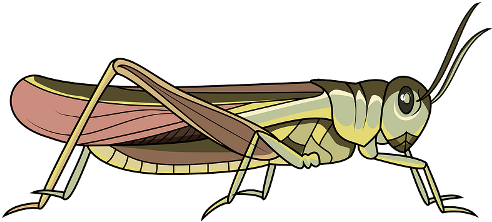
\includegraphics{locusta}
    \caption{locusta, -ae (f)}
\end{figure}%
ego indūcam crās locustam in\linebreak fīnēs tuōs:  quæ operiat
\mpp{superficiēs, -eī (f)}{pars superior vel summa alicuius reī}superficiem terræ, nē quidquam eius appāreat, sed
\mpp{comedere:}{totum ēsse; ēsse}comedātur quod \mpp{residuus/a/um:}{quod reliquum est}residuum
fuerit \mpp{grandō, grandinis (f):}{aqua frigidissima lapidī similis quae cadit dē
caelō}grandinī: \mpp{corrōdere:}{consumere}corrōdet enim omnia ligna quæ
\mpp{germinare:}{emittere germina (ea quae ex herbis veniunt semen,
fructus, cet.)}germinant in agrīs.  Et implēbunt domōs tuās, et servōrum
tuōrum, et omnium Ægyptiōrum, quantam nōn vīdērunt patrēs tuī, et \mpp{avus, -ī (m):}{pater patris vel matris}avī, ex
quō ortī sunt super terram, usque in præsentem diem. 

Āvertitque sē, et
ēgressus est ā Pharaōne.  Dīxērunt autem servī
Pharaōnis ad eum: \mpp{usquequō:}{usque ad quod tempus?}``Usquequō patiēmur hoc
\mpp{scandalum, -ī (n):}{rēs perdita}scandalum? Dīmitte hominēs, ut sacrificent Dominō Deō suō;
nōnne vidēs quod perierit Ægyptus?''

Revocāvēruntque Moysen et Aarōn ad
Pharaōnem, quī dīxit eīs: ``Īte, sacrificātē Dominō Deō vestrō: quīnam
sunt quī itūrī sunt?''

Ait Moysēs: ``Cum parvulīs nostrīs, et seniōribus
pergēmus, cum fīliīs et fīliābus, cum ovibus et \mpp{armentum, -ī (n):}{maiorum bestiarum grex (e.g: equōrum, bovum)}armentīs:
est enim \mpp{sōlemnitās, -ātis (f):}{diēs quī certīs temporibus quotannis fit quō homines deum servunt}sōlemnitās Dominī Deī nostrī.''

Et respondit
Pharaō: ``Sīc Dominus sit vōbīscum, quōmodo ego dīmittam
vōs, et parvulōs vestrōs, cui dubium est quod pessimē cōgitētis?  Nōn
fīet ita, sed īte tantum virī, et sacrificātē Dominō: hoc enim et ipsī
petīstis.''

Statimque ēiectī sunt dē cōnspectū Pharaōnis.  Dīxit autem
Dominus ad Moysēn: ``Extende manum tuam super terram Ægyptī ad locustam, ut
ascendat super eam, et dēvoret omnem herbam quæ \mpp{residuus/a/um:}{quod reliquum est}residua
fuerit \mpp{grandō, grandinis (f):}{aqua frigidissima lapidī similis quae cadit dē caelō}grandinī.''

Et extendit Moysēs virgam super terram Ægyptī: et
Dominus indūxit ventum ūrentem tōtā diē illā et nocte: et manē factō,
ventus ūrēns levāvit locustās.  Quæ ascendērunt super
ūniversam terram Ægyptī: et sēdērunt in cūnctīs fīnibus Ægyptiōrum
\mpp{innumerābilis, -e (adj):}{quī numerārī nōn potest}innumerābilēs, quālēs ante illud tempus nōn fuerant, nec
posteā futūræ sunt.  Operuēruntque ūniversam superficiem terræ,
\mpp{vastāre:}{percutere}vastantēs omnia. Dēvorāta est igitur herba terræ, et
quidquid \mimg{poma}{pōma\\pōmum, -ī (n)}pōmōrum in arboribus fuit, quæ grandō dīmīserat:
nihilque \mpp{omnino:}{vere, certe}omnīnō virēns relictum est in lignīs et
in herbīs terræ, in cūnctā Ægyptō.

Quam ob rem \mpp{festīnus/a/um:}{celeriter aliquid agens}festīnus
Pharaō vocāvit Moysen et Aarōn, et dīxit eīs: ``\mpp{peccatum:}{res contra
legem acta}Peccāvī in Dominum Deum vestrum, et in vōs.  Sed nunc
dīmittite peccātum mihi etiam hāc vice, et rogātē Dominum Deum vestrum, ut
auferat ā mē mortem istam.''

Ēgressusque Moysēs dē cōnspectū Pharaōnis,
ōrāvit Dominum.  Quī flāre fēcit ventum ab occidente
\mpp{vehemēns, -entis (adj):}{ferox, iratus, severus}vehementissimum, et \mpp{arripere:}{vī prehendere}arreptam locustam
prōiēcit in mare Rubrum: nōn remānsit nē ūna quidem in cūnctīs fīnibus
Ægyptī.  Et indūrāvit Dominus cor Pharaōnis, nec dīmīsit fīliōs
Isrāēl.  

Dīxit autem Dominus ad Moysēn: ``Extende manum
tuam in cælum: et sint tenebræ super terram Ægyptī tam
\mpp{densus/a/um:}{cuius partēs inter sē premunt}dēnsæ, ut \mpp{palpārī:}{leviter tangere}palpārī \mpp{queant =}{possint}queant.''

Extenditque
Moysēs manum in cælum: et factæ sunt tenebræ \mpp{horribilis, -e (adj):}{timendus/a/um}horribilēs in
ūniversā terrā Ægyptī tribus diēbus.  Nēmō vīdit frātrem suum, nec mōvit
sē dē locō in quō erat: \mpp{ubicumque:}{in omne locō in quō...}ubicumque autem habitābant fīliī
Isrāēl, lūx erat.

Vocāvitque Pharaō Moysen et Aarōn, et dīxit eīs: ``Īte,
sacrificātē Dominō: ovēs tantum vestræ et \mpp{armentum, -ī (n):}{maiorum bestiarum grex (e.g: equōrum, bovum)}armenta
remaneant, parvulī vestrī eant vōbīscum.''

Ait Moysēs: ``Hostiās quoque et
\mpp{holocaustum:}{sacrificium igne factum}holocausta dabis nōbīs, quæ offerāmus Dominō Deō nostrō. 
Cūnctī gregēs pergent nōbīscum; nōn remanēbit ex eīs
\mimg{hoof}{ungula, -ae (f)}ungula: quæ necessāria sunt in \mpp{cultus, -ūs (m):}{cura Deī}cultum Dominī Deī nostrī:
\mpp{praesertim:}{praecipue}præsertim cum ignōrēmus quid dēbeat
\mpp{immolāre:}{sacrificium facere}immolārī, dōnec ad ipsum locum
perveniāmus.''

Indūrāvit autem Dominus cor Pharaōnis, et nōluit dīmittere
eōs.  Dīxitque Pharaō ad Moysēn: ``Recēde ā mē, et cave nē ultrā videās
faciem meam: quōcumque diē appārueris mihi, moriēris.''

Respondit Moysēs: ``Ita fīet ut locūtus es: nōn vidēbō ultrā faciem tuam.''


\chapter{}

\titleimg{firstborn_title}

\mktitle{Capitulum Undecimum}
\thispagestyle{empty}

\cstart{E}{t} dīxit Dominus ad Moysēn: ``Adhūc ūnā
\mpp{plaga, ae (f):}{e.g, unus pulsat alterum; eo tempore cum pugnus corpus tangit
`plaga' vocatur}plāgā tangam Pharaōnem et Ægyptum, et post
hæc dīmittet vōs, et exīre \mpp{compellere:}{vī facere ut aliquis aliquid agat}compellet. \vnum{2}Dīcēs ergō omnī
\mpp{plēbs, plēbis (f):}{populus; praecipue hominēs quī pecuniosī non sunt ac minimam potestatem habent}plēbī ut postulet vir ab amīcō suō, et mulier ā
\mpp{vīcīnus/a/um:}{quī vel quae prope habitat}vīcīnā suā, vāsa argentea et aurea. \vnum{3}Dabit autem Dominus
grātiam populō suō cōram Ægyptiīs.''

Fuitque Moysēs vir
magnus valdē in terrā Ægyptī cōram servīs Pharaōnis et omnī
populō. \vnum{4}Et ait: ``Hæc dīcit Dominus: Mediā nocte ēgrediar in Ægyptum: 
\vnum{5}et moriētur omne \mpp{prīmōgenitus/a/um:}{quī vel quae prīmus natus est}prīmōgenitum in terrā Ægyptiōrum, ā
prīmōgenitō Pharaōnis, quī sedet in soliō eius, usque ad
prīmōgenitum ancillæ quæ est ad \mpp{mola, -ae (f):}{instrumentum grave quō frumentum premitur in minimās partēs}molam, et omnia
prīmōgenita \mpp{iumentum, -ī (n):}{animal utile ad gerendum vel
trahendum e.g, equi, boves, et cetera}iūmentōrum. \vnum{6}Eritque clāmor magnus
in ūniversā terrā Ægyptī, quālis nec ante fuit, nec posteā futūrus est. 
\vnum{7}Apud omnēs autem fīliōs Isrāēl nōn \mpp{mūtīre:}{parvā voce sonum facere vel loquī}mūtiet
canis ab homine usque ad pecūs: ut sciātis quantō \mpp{mīrāculum, -ī
(n):}{opus optime factum quod admirationem afferre potest}mīrāculō
dīvidat Dominus Ægyptiōs et Isrāēl. \vnum{8}Dēscendentque omnēs servī tuī istī ad
mē, et adōrābunt mē, dīcentēs: Ēgredere tū, et omnis populus quī
\mpp{subicere:}{facere ut aliquis alicui pareat}subiectus est tibi: post
hæc ēgrediēmur.''

\vnum{9}Et exīvit ā Pharaōne īrātus nimis. Dīxit
autem Dominus ad Moysēn: ``Nōn audiet vōs Pharaō ut multa
signa fīant in terrā Ægyptī.''

\vnum{10}Moysēs autem et Aarōn fēcērunt omnia
ostenta, quæ scrīpta sunt, cōram Pharaōne. Et \mpp{indurare:}{durum
facere}indūrāvit Dominus cor Pharaōnis, nec dīmīsit fīliōs Isrāēl dē terrā
suā. 


\chapter{}

\titleimg{birdhead}

\mktitle{Capitulum Duodecimum}
\thispagestyle{empty}

\vnum{1}Dīxit quoque Dominus ad Moysēn et Aarōn in terrā
Ægyptī: \vnum{2}``Mēnsis iste, vōbīs prīncipium mēnsium: prīmus erit in mēnsibus
annī. \vnum{3}Loquiminī ad ūniversum \mpp{cœtus, -ūs (m):}{grex hominum}\mimg{babygoat}{haedus, -ī (m)}cœtum fīliōrum Isrāēl, et
dīcite eīs: Decima diē mēnsis huius tollat ūnusquisque agnum per familiās
et domōs suās. \vnum{4}Sīn autem minor est numerus ut \mpp{sufficere:}{satis esse}sufficere
possit ad \mpp{vēscī:}{ēsse}vēscendum agnum, assūmet \mpp{vicinus/a/um:}{prope habitans}vīcīnum suum quī iūnctus est domuī suæ, iuxtā numerum
animārum quæ sufficere possunt ad ēsum agnī.''

\vnum{5}``Erit autem agnus absque
\mpp{macula, -ae (f):}{pars in quā proprius color abest}maculā,
\mpp{masculus/a/um:}{masculīnus}masculus, \mpp{anniculus/a/um:}{unius annī}anniculus:
iuxtā quem \mpp{rītus, -ūs (m):}{res agendae ut sacra recte fiant}rītum
tollētis et hædum. \vnum{6}Et
servābitis eum usque ad quartamdecimam diem mēnsis huius:
\mpp{immolare:}{sacrificium facere}immolābitque eum ūniversa multitūdō
fīliōrum Isrāēl ad \mpp{vespera, -ae (f) =}{vesper}vesperam.''

\begin{figure}[h!]
    \begin{minipage}[hp]{0.5\linewidth}
        \centering
        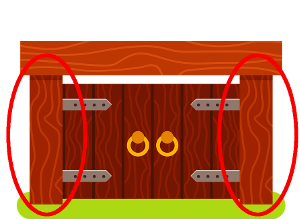
\includegraphics{postis}
        \caption{postis, -is (m)}
    \end{minipage}%
    \begin{minipage}[hp]{0.5\linewidth}
        \centering
        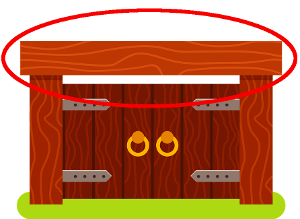
\includegraphics{superlimen}
        \caption{superlīmināre, -is (n)}
    \end{minipage}
\end{figure}

\vnum{7}``Et sūment dē sanguine eius,
ac pōnent super utrumque postem, et in
superlīmināribus \mimg{lactuca}{lactūca, -ae (f)}domōrum, in quibus \mpp{comedere:}{totum
esse; esse}comedent illum. \vnum{8}Et edent carnēs nocte illā
\mpp{assus/a/um}{sine aquā vel aliā materiā fluentī coctus}assās ignī, et
\mpp{azȳmus/a/um:}{sine materiā quae efficit ut panis turgidus fiat}azȳmōs pānēs cum lactūcīs \mpp{agrestis, -e (adj) <}{ager}agrestibus. \vnum{9}Nōn
comedētis ex eō \mpp{crūdus/a/um:}{non coctus}crūdum quid, nec coctum aquā, sed tantum
assum ignī: caput cum pedibus eius et intestīnīs
vorābitis.''

\begin{figure}[h!]
    \begin{minipage}[hp]{0.5\linewidth}
        \centering
        
\includegraphics{intestine}
        \caption{intestīnus, -ī (m)}
    \end{minipage}%
    \begin{minipage}[hp]{0.5\linewidth}
        \centering
        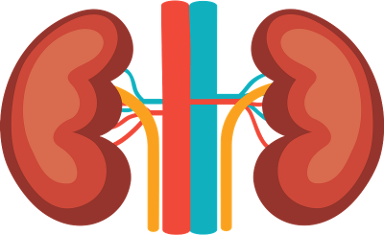
\includegraphics{renes}
        \caption{rēnēs, rēnum (m)}
    \end{minipage}
\end{figure}

\vnum{10}``Nec remanēbit quidquam ex eō usque manē; sī quid
\mpp{residuus:}{quod reliquum est}residuum fuerit, igne
\mpp{comburere:}{igne perdere}combūrētis. \vnum{11}Sīc autem comedētis illum:
\mpp{rēnēs accingere:}{induere vestis quae cingit corpus circiter rēnēs}rēnēs vestrōs \mpp{accingere =}{cingere}accingētis, et
\mpp{calceamentum:}{quod pedi induitur}calceāmenta habēbitis in pedibus,
tenentēs baculōs in manibus, et comedētis \mpp{festīnanter =}{celeriter}festīnanter: est
enim \mpp{Phase:}{vocabulum Hebraicum ``trānsitus'' significans}Phase (id est, trānsitus) Dominī. \vnum{12}Et trānsībō per
terram Ægyptī nocte illā, percutiamque omne \mpp{prīmōgenitus/a/um:}{quī vel quae prīmus natus est}prīmōgenitum in
terrā Ægyptī ab homine usque ad pecūs: et in cūnctīs dīīs Ægyptī faciam
\mpp{iūdicium, -ī (n):}{quod iudex tradit}\mimg{judge_small}{iudex, iudicis (m/f)}iūdicia. Ego Dominus. \vnum{13}Erit autem sanguis vōbīs in signum
in \mpp{aedēs, aedium (f pl.):}{aedificium}ædibus in quibus eritis: et vidēbō sanguinem, et
trānsībō vōs: nec erit in vōbīs \mpp{plāga, -ae (f):}{e.g, unus pulsat alterum eo
tempore cum pugnus corpus tangit `plāga' vocatur}plāgā
\mpp{disperdere:}{valde perdere}disperdēns quandō percusserō terram Ægyptī. \vnum{14}Habēbitis
autem hunc diem in \mpp{monumentum, -ī (n):}{quiquid nōs monet}monumentum: et
\mpp{celebrāre:}{agere quod oportet agere die Deō constitutō}celebrābitis eam \mpp{sōlemnis, -e (adj):}{sōlemnis dicitur de rēbus deō constitutibus quae certīs temporibus quotannis fit}sōlemnem Dominō in
\mpp{generātio, -ōnis (f):}{e.g: una generatio parentibus constat, līberīs eōrum altera generatio constat, etc...}generātiōnibus vestrīs cultū \mpp{sempiternus/a/um:}{perpetuus}sempiternō.
\vnum{15}Septem diēbus azȳma comedētis: in diē prīmō nōn erit
\mpp{fermentum, -ī (n):}{materia quae efficit ut panis turgidus fiat}fermentum in domibus vestrīs: quīcumque comēderit
\mpp{fermentō, -āre, -āvī, -ātum:}{ponere fermentum in aliquō}fermentātum, perībit anima illa dē Isrāēl, ā prīmō diē
usque ad diem septimum.''

\vnum{16}``Diēs prīma erit \mpp{sānctus/a/um:}{deō pertinens}sāncta atque
sōlemnis, et diēs septima eādem \mpp{fēstīvitās, -ātis (f):}{dies laetus deō constitutus}fēstīvitāte
\mpp{venerābilis, -e (adj):}{cultū dignus}venerābilis: nihil operis faciētis in eīs,
\mpp{exceptīs hīs:}{praeter hās}exceptīs hīs, quæ ad vēscendum \mpp{pertinere:}{e.g, colloquium ad me pertinet si homines loquuntur de me}pertinent. \vnum{17}Et
\mpp{observābitis azȳma:}{quotannis diem sanctam celebrētis in quā azymī panēs comeduntur}observābitis azȳma: in eādem enim ipsā diē ēdūcam
exercitum vestrum dē terrā Ægyptī, et cūstōdiētis diem istum in
generātiōnēs vestrās \mpp{rītus, -ūs (m):}{res agendae ut sacra recte fiant}rītū perpetuō.  \vnum{18} Prīmō mēnse, quartadecīmā diē mēnsis ad vesperam, comedētis
azȳma usque ad diem \mpp{vīgēsimam =}{vīcēsimam}vīgēsimam prīmam eiusdem mēnsis ad
vesperam. \vnum{19}Septem diēbus fermentum nōn inveniētur in domibus vestrīs:
quī comēderit fermentātum, perībit anima eius dē cœtū Isrāēl, tam dē
\mpp{advena, -ae (m)}{qui non est civis, qui ab alio loco venit}advenīs quam dē \mpp{indigena, -ae (adj)}{natus in eō lōcō}indigenīs terræ. \vnum{20}Omne fermentātum nōn
comedētis: in cūnctīs \mpp{habitāculum, -ī (n):}{locus in quō aliquis habitat}habitāculīs vestrīs edētis azȳma.''

\vnum{21}Vocāvit autem Moysēs omnēs seniōrēs fīliōrum Isrāēl, et
dīxit ad eōs: ``Īte tollentēs animal per familiās vestrās, et immolātē
Phase. \vnum{22}\mpp{fasciulum, -ī:}{multum lignī vel materiae aliae vinctum}Fasciculumque \mpp{hyssōpum, -ī (n):}{herba quaedam}hyssōpī
\mpp{tingere:}{humidum facere}tingite in sanguine quī est in līmine, et aspergite ex eō
superlīmināre, et utrumque postem: nūllus vestrum
ēgrediātur ōstium domūs suæ usque manē. \vnum{23}Trānsībit enim Dominus
percutiēns Ægyptiōs: cumque vīderit sanguinem in
superlīminārī, et in utrōque poste,
\mpp{trānscendere:}{transīre}trānscendet ōstium domūs, et nōn sinet
\mpp{percussōr, -ōris (m):}{quī percutit}percussōrem \mpp{ingredi:}{intus ire}ingredī domōs vestrās
et lædere. \vnum{24}Cūstōdī verbum istud \mpp{lēgitimus/a/um:}{qui secundum legēs est; iustus; verus}lēgitimum tibi et fīliīs
tuīs usque in \mpp{in aeternum:}{semper}æternum. \vnum{25}Cumque \mpp{introire:}{intus ire;
ingredi}introierītis terram, quam Dominus datūrus est vōbīs ut pollicitus
est, observābitis \mpp{cæremōnia, ae (f):}{res agendae ut sacra recte fiant}cæremōniās istās. \vnum{26}Et cum dīxerint
vōbīs fīliī vestrī: Quæ est ista \mpp{religiō, -ōnis (f):}{rītus}religiō? \vnum{27}Dīcētis eīs:
\mpp{victima, -ae (f):}{animal sacrificiō statutum}Victima trānsitūs Dominī est, quandō trānsīvit super
domōs fīliōrum Isrāēl in Ægyptō, percutiēns Ægyptiōs, et domōs nostrās
līberāns.''

\mimg{scimitar}{gladius \emph{incurvātus}}Incurvātusque populus adōrāvit. \vnum{28}Et ēgressī
fīliī Isrāēl fēcērunt sīcut \mpp{praecipere:}{imperare}præcēperat Dominus
Moȳsī et Aarōn. \vnum{29}Factum est autem in noctīs mediō, percussit Dominus omne
\mpp{prīmōgenitus/a/um:}{quī vel quae prīmus natus est}prīmōgenitum in terrā Ægyptī, ā prīmōgenitō
Pharaōnis, quī in soliō eius sedēbat, usque ad prīmōgenitum
\mpp{captīvus/a/um:}{qui captus, qui vinctus est}captīvæ quæ erat in carcere, et omne prīmōgenitum
\mpp{iumentum:}{animal utile ad gerendum vel trahendum e.g, equi, boves, et
cetera}iūmentōrum. \vnum{30}Surrēxitque Pharaō nocte, et omnēs
servī eius, cūnctaque Ægyptus: et ortus est clāmor magnus in Ægyptō:
neque enim erat domus in quā nōn iacēret mortuus. 

\vnum{31}Vocātīsque Pharaō
Moyse et Aarōn nocte, ait: ``Surgite et ēgrediminī ā populō
meō, vōs et fīliī Isrāēl: īte, immolātē Dominō sīcut dīcitis. \vnum{32}Ovēs
vestrās et \mpp{armentum, -ī (n):}{maiorum bestiarum grex (e.g: equōrum, bovum)}armenta assūmite ut petierātis, et abeuntēs
\mpp{benedīcere:}{sanctum facere}benedīcite mihi.''

\vnum{33}\mpp{urgēre:}{valde hortārī; cogere}Urgēbantque Ægyptiī
populum dē terrā exīre vēlōciter, dīcentēs: ``Omnēs moriēmur.''

\vnum{34}Tulit
igitur populus \mpp{cōnspergō, cōnspergere, cōnspersī, conspersum:}{spargere}cōnspersam \mpp{farīna, -ae (f):}{materia, aquā impositā, ex quā panis factus est}farīnam antequam
\mpp{fermentō, -āre, -āvī, -ātum:}{ponere fermentum in aliquō}fermentārētur: et ligāns in palliīs, posuit super
\mpp{humerōs =}{umerōs}humerōs suōs. \vnum{35}Fēcēruntque fīliī Isrāēl sīcut præcēperat
Moysēs: et petiērunt ab Ægyptiīs vāsa argentea et aurea, vestemque
plūrimam. \vnum{36}Dominus autem dedit grātiam populō cōram Ægyptiīs ut
\mpp{commodāre:}{libenter cum aliquō facere, libenter rēs dāre}commodārent eīs: et \mpp{spoliare:}{capere res aliorum
hominum}spoliāvērunt Ægyptiōs. 

\vnum{37}Profectīque sunt fīliī Isrāēl dē Ramesse
in Socoth, sexcenta ferē mīllia peditum virōrum, absque parvulīs. \vnum{38}Sed et
\mpp{vulgus, -ī (n):}{multitudo, turba}vulgus \mpp{prōmiscuus/a/um:}{mixtum}prōmiscuum \mpp{innumerabilis:}{qui
numerari non potest}innumerābile ascendit cum eīs, ovēs et armenta et
animantia \mpp{diversus:}{in varias partes versi sunt}dīversī generis multa
nimis. \vnum{39}Coxēruntque farīnam, quam \mpp{dūdum:}{nuper}dūdum dē Ægyptō
cōnspersam tulerant: et fēcērunt \mpp{subcinerīcus pānis:}{panis sub cinere coctus}subcinerīciōs pānēs
azȳmōs: neque enim poterant fermentārī, cōgentibus exīre
Ægyptiīs, et nūllam facere sinentibus moram: nec \mpp{pulmentum, -ī (n):}{cibus}pulmentī
quidquam occurrerat \mpp{praeparāre:}{parāre, ante parāre}præparāre.

\vnum{40}\mpp{habitātiō, -ōnis (f)}{actus habitandī}Habitātiō
autem fīliōrum Isrāēl quā mānsērunt in Ægyptō, fuit quadringentōrum
trīgintā annōrum. \vnum{41}Quibus \mpp{explere:}{perficere}explētīs, eādem diē
ēgressus est omnis exercitus Dominī dē terrā Ægyptī. \vnum{42}Nox ista est
\mpp{observāre:}{colere, servāre}\mpp{observābilis, -e (adj):}{quod potest observārī}observābilis Dominī, quandō ēdūxit eōs dē terrā Ægyptī: hanc
observāre dēbent omnēs fīliī Isrāēl in generātiōnibus suīs.

\vnum{43}Dīxitque Dominus ad Moysēn et Aarōn: ``Hæc est religiō Phase: omnis
\mpp{aliēnigena, -ae (m/f):}{aliō locō natus}aliēnigena nōn comedet ex eō. \vnum{44}Omnis autem servus
\mpp{emptitius =}{emptus}emptitius \mpp{circumcīdere:}{Removēre secandō summum membrum inter crura puerī vel virī situm}circumcīdētur, et sīc comedet. \vnum{45}Advena et
\mpp{mercēnārius, -ī (m):}{cui merces datur ut opus faciat}mercēnārius nōn edent ex eō. \vnum{46}In ūnā domō comedētur, nec
\mpp{efferre:}{extra ferre, proferre}efferētis dē carnibus eius forās, nec os illīus
\mpp{confringere:}{una frangere}cōnfringētis. \vnum{47}Omnis \mpp{cœtus, -ūs (m):}{grex hominum}cœtus fīliōrum
Isrāēl faciet illud. \vnum{48}Quod sī quis \mpp{peregrīnus/a/um:}{quī ex aliā terrā vēnit}peregrīnōrum in
vestram voluerit trānsīre \mpp{colōnia, -ae (f):}{locus in quō hominēs domūs novās confēcērunt et agrōs colere incēpērunt}colōniam, et facere Phase Dominī,
circumcīdētur prius omne masculīnum eius, et tunc \mpp{rītus, -ūs (m):}{res agendae ut sacra recte fiant}rīte
celebrābit: eritque sīcut \mpp{indigena, -ae (adj)}{natus in eō lōcō}indigena terræ:
sī quis autem circumcīsus nōn fuerit, nōn
\mpp{vēscī:}{ēsse}vēscētur ex eō. \vnum{49}Eādem lēx erit indigenæ
et colōnō quī \mpp{peregrinārī:}{iter facere per aliēna loca, patria procul abīre}peregrīnātur apud vōs.''

\vnum{50}Fēcēruntque omnēs
fīliī Isrāēl sīcut præcēperat Dominus Moȳsī et Aarōn. \vnum{51}Et eādem diē
ēdūxit Dominus fīliōs Isrāēl dē terrā Ægyptī per \mpp{turma, -ae (f):}{multitūdō}turmās
suās. 


\chapter{}
% \newgeometry{top=0.75in, bottom=1.0in, outer=1.75in, inner=0.4in, heightrounded, 
% marginparwidth=3.5cm, marginparsep=0.5cm}

\newgeometry{top=0.75in, bottom=3cm, outer=3cm, inner=3cm}

\pagestyle{fancy}
\fancyhead{}
\chead{}
%\rhead{\thechapter}
\cfoot{} % get rid of the page number
\renewcommand{\headrulewidth}{1pt}
\renewcommand{\footrulewidth}{0pt}
{\tiny
    \begin{flushleft}
    \twocolumn
    \parskip 0.5ex
    \setlength{\parindent}{0pt}
    \input{lexicon.tex}
    \end{flushleft}
}

\end{document}
